\section*{Learning Objectives}
\begin{itemize}
\item Extend our horizons from linear equations to nonlinear equations. 
\item Appreciate the power of using algorithms to iteratively construct approximate solutions to a problem.
\item Accomplish all of this without assuming a background in Calculus.
\end{itemize}

\section*{Outcomes}
\begin{itemize}
\item Learn that a root is a solution of an equation of the form $f(x)=0$.
\item Learn two methods for finding roots of real-valued functions of a real variable, that is for $f:\real \to \real$, namely the Bisection Method and Newton's Method
\item Become comfortable with the notion of a ``local slope'' of a function at a point and how to compute it numerically.
\item Linear approximations of nonlinear functions.
\item Extensions of these ideas to vector-valued functions of several variables, that is $f:\real^m \to \real^n$, with key notions being the gradient and Jacobian of a function and their use in the Newton-Raphson Algorithm.
\end{itemize}


\vspace*{1.5cm}





\newpage

\section{Motivation and Simple Ideas}

The focus of ROB 101 has been systems on linear equations. Long before you came to ROB 101, however, you had studied some Algebra and solved a few nonlinear equations. Our goal here is to develop numerical methods for finding solutions to \textbf{systems of nonlinear equations}. \\

We will limit our notion of a solution to the set of real numbers or real vectors. Limiting our search for solutions to the real numbers has consequences. We already know that 
$$x^2 + 1=0, $$
for example, has no real solutions because its discriminant is $\Delta = b^2-4 ac = - 4 <0$. Nevertheless, many interesting problems in Engineering and Science can be formulated and solved in terms of ``real solutions'' to systems of equations\footnote{In addition, we should not overlook the fact that as a first introduction to the subject of numerical methods for solving systems of nonlinear equations, working with real numbers and vectors is a great place to start!}. \\

\begin{tcolorbox}[title=\textbf{Root of an Equation}]
 Let $f:\real^n \to \real$ be a function. Then $f(x)=0$ defines an equation. A solution to the equation is also called a \textbf{root}\footnote{In the 9th century, Arab writers usually called one of the solutions to a polynomial equation \textbf{jadhr} (“root”), and their medieval European translators used the Latin word \textbf{radix}; see \url{https://www.britannica.com/science/root-mathematics}.}; that is $x^\ast \in \real^n$ is a root of $f(x)=0$ if
\begin{equation}
    \label{eq:DefRoot}
    f(x^\ast)=0.
\end{equation}
Just as with quadratic equations, it is possible that \eqref{eq:DefRoot} has multiple real solutions or no real solutions.\\

You may wonder if we could seek solutions to $f(x)=\pi$, for example, and if we were to do that, would we still call them roots? Technically, the answer is no. The term root is reserved for solutions to $f(x)=0$. However, if we define a new function, $\bar{f}(x):=f(x)-\pi,$ then 
$$\bar{f}(x^\ast)=0 \iff  f(x^\ast)-\pi = 0 \iff f(x^\ast) = \pi,$$
and $x^\ast$ is a root of our new function $\bar{f}(x)$. If this seems like we are splitting hairs, yeah, it's hard to disagree with that sentiment!
\end{tcolorbox}

    
    \begin{figure}[htb]%
\centering
\subfloat[]{%
    \label{fig:Continuous}%
	\centering
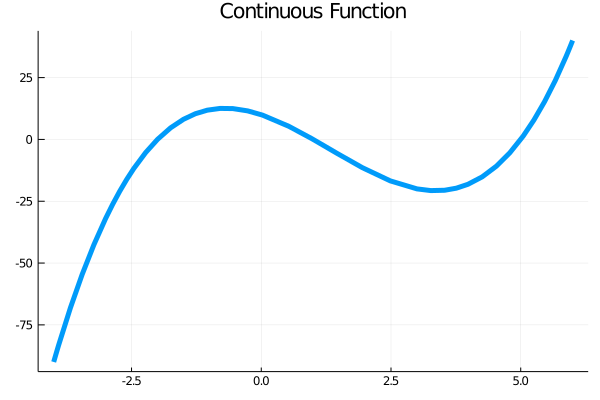
\includegraphics[width=0.3\columnwidth]{Chap11NonlinearEquations/ContinuousNotContinuousA.png}}%
\hspace{5pt}%
\subfloat[]{%
    \label{fig:Discontinuous}%
	\centering
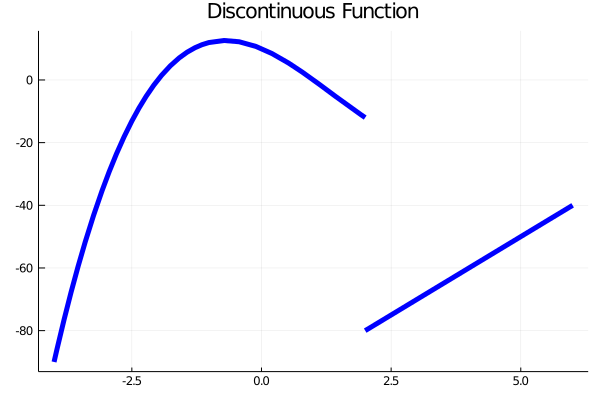
\includegraphics[width=0.3\columnwidth]{Chap11NonlinearEquations/ContinuousNotContinuousB.png}}%
\hspace{5pt}%
\subfloat[]{%
    \label{fig:NotFunction}%
	\centering
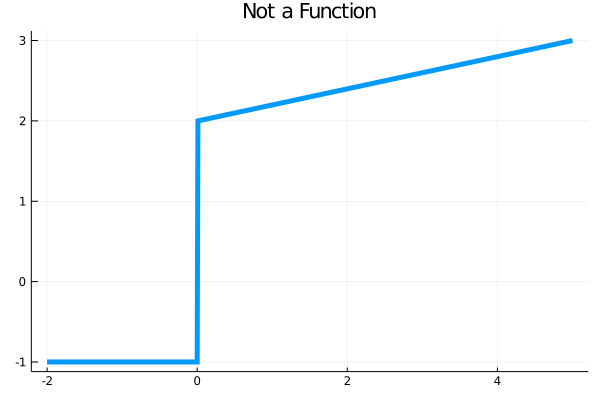
\includegraphics[width=0.3\columnwidth]{Chap11NonlinearEquations/ContinuousNotContinuousC.png}}%
    \caption[]{Examples of a continuous function, a discontinuous function, and a graph that is not a function. Yes, in (c), the point $x=0$ is mapped to the interval $[-1, 2]$. To be a function, each point in the domain can only map to a single point in the range. }
    \label{fig:ContinuousVsNot}
\end{figure}

 We will say very informally that a function $f:\real \to \real$ is \textbf{continuous} if you can draw the graph of $y=f(x)$ on a sheet of paper without lifting your pencil (from the paper)! Figure~\ref{fig:ContinuousVsNot}-(a) clearly passes this test while Fig.~\ref{fig:ContinuousVsNot}-(b) does not. Figure~\ref{fig:ContinuousVsNot}-(c) ``seems'' to pass the ``without lifting your pencil test,'' but the graph does not represent a function! Recall that a function is a rule that associates to each element of the domain, a single value in the range, meaning, that for a given $x\in \real$, there can be only one value of $y\in \real$ such that $y=f(x)$. In Fig.~\ref{fig:ContinuousVsNot}-(c), for $x=0$, we have $f(x)=y$ for all $y\in [-1, 2]$, which makes it not a function. What about the part of the graph where the ``non-function'' is constant, does that also make it not a function? No, it is fine for the single value of $y=-1.0$ to be associated with many values of $x$; it's the other way around that is a problem. Functions map points to points and not points to non-trivial sets, such as the interval $[-1, 2]$. \\
 
 In Calculus, you will encounter a formal definition, which goes something like this:   $f:\real \to \real$ is \textbf{continuous at a point $\mathbf{ x_0 \in \real}$} if for every $\epsilon>0$, there exists a $\delta >0$ such that, $$ |x-x_0| < \delta \implies |f(x)-f(x_0)| < \epsilon.$$ 
 And then one says that $f$ is \textbf{continuous} if it is continuous at $x_0$ for all $x_0$ in its domain of definition! 
 For our purposes, the pencil test is good enough.






\section{Bisection}
\label{sec:BisectionAlgorithm}

We begin with the most straightforward and intuitive method for finding roots of scalar equations $$f(x)=0, $$
where $f:\real \to \real,$ that is, $f$ maps real numbers to real numbers. The method is based on the following fact, which, once again, is something you will encounter in Calculus. In ROB 101, we are giving you a reason to pay attention to the result when it is presented in Calculus! 

\vspace*{0.5cm}
\begin{tcolorbox}[sharp corners, colback=green!30, colframe=green!80!blue, title=\textbf{\large Intermediate Value Theorem}]
Assume that $f$ is a continuous real valued function and you know two real numbers $a < b$ such that $f(a) \cdot f(b) <0$. Then there exists a real number $c$ such that
\begin{itemize}
    \item $a < c < b$~~ ($c$ is between $a$ and $b$), and
    \item $f(c)=0$~~ ($c$ is a root).
\end{itemize}
The values $a$ and $b$ are said to \textbf{bracket the root}, $c$. 
\end{tcolorbox}

Remarkably, this leads to a ``method'' for approximating roots with arbitrary accuracy! Here is the basic idea.

\begin{tcolorbox}[title=\textbf{\large Bisection Algorithm Pseudo Code}]
\begin{itemize}
\item \textbf{Initialize}: define $a < b$ such that $f(a) \cdot f(b) < 0$
    \item \textbf{Start}: compute $c:=\frac{a+b}{2}$, the midpoint of the interval $[a, b]$. 
    \item Two things are possible: 
    \begin{itemize}
    \setlength{\itemsep}{.2cm}
        \item $f(c)=0$, in which case, we are done. $x^\ast=c.$
        \item $f(c) \neq 0$, in which case, \textbf{either} $f(c) \cdot f(a) < 0$ \textbf{or} $f(c) \cdot f(b) < 0$. (We'll leave to you the task of ``proving'' that at least one of these statements must be true and they cannot both be true.)
                    
    \end{itemize}
        \item \textbf{If}  $f(c) \cdot f(a) < 0$\\
        \hspace*{.3cm}$b =c;$  ~~\# $b$ updates while $a$ stays the same\\
        \textbf{Else}\\
        \hspace*{.3cm} $a =c$;  ~~\# $a$ updates while $b$ stays the same\\
        \textbf{End If}\\
        \item  \textbf{Loop Back to Start.} ( \textit{Wash, rinse, and repeat!} )
\end{itemize}
\end{tcolorbox}

Now, as written, the above is not an effective algorithm because it may never terminate, meaning it could loop for ever and ever. For example, suppose you wanted to solve $x^2-2 = 0$. You know that answer is $x^\ast=\sqrt{2}$, an irrational number. You might think to start with the initial guesses being $a=0$ and $b=2$, because then $f(0) \cdot f(2) = (-2) \cdot (2) = -4 <0$. However, $c=\frac{a+b}{2} =1$, a rational number, and because $f(c) \cdot f(b)<0$, your next step is $a=1$ and $b=2$. In fact, you can check that $[a ~~c ~~b]$ evolves like this
\begin{align*}
\begin{array}{lll}
~a & ~c & ~b\\
0.0 & 1.0 & 2.0 \\
1.0 & 1.5 & 2.0 \\
1.0 & 1.25 & 1.5 \\
1.25 & 1.375 & 1.5 \\
1.375 & 1.4375 & 1.5 \\
1.375 & 1.40625 & 1.4375 \\
1.40625 & 1.421875 & 1.4375 \\
1.40625 & 1.4140625 & 1.421875 \\
1.4140625 & 1.41796875 & 1.421875 \\
1.4140625 & 1.416015625 & 1.41796875 \\
1.4140625 & 1.4150390625 & 1.416015625 
\end{array}
\end{align*}
the point being that $c$ will always be a rational number and hence it will never be true that $f(c)=0.$ Of course, we can get very close to zero and we need to define what does close enough mean!

   \begin{figure}[hbt!]
    \centering
    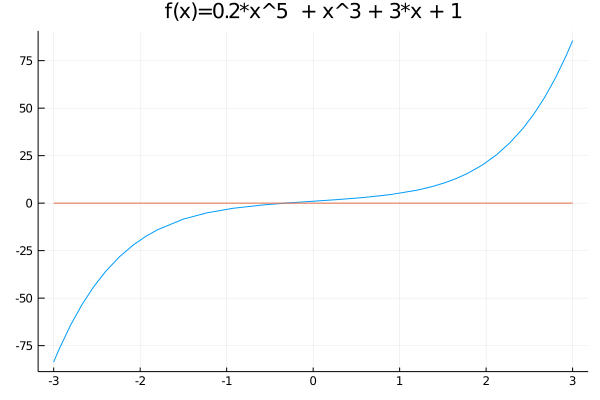
\includegraphics[scale=0.5]{Chap11NonlinearEquations/BisectionExample0.png}
    \caption[]{Plot of $y=0.2x^5  + x^3 + 3x + 1$. There does not exist any formula that provides the roots of general quintic polynomials (no quintic equation)! If we want to find a root, we are forced to use numerical methods.}
    \label{fig:BisectionExample1a}
    \end{figure}
    
\begin{example}
\label{ex:Bisection} 

Figure~\ref{fig:BisectionExample1a} presents a graph of the function $f(x)=0.2x^5  + x^3 + 3x + 1$. Find a root of the function, that is, find a solution of
$$0.2x^5  + x^3 + 3x + 1=0. $$
Because formulas for the roots of quintic polynomials do not exist\footnote{In fact, N. Abel proved in 1826 that formulas for roots do not exist for families of polynomials of degree higher than four. In 1835, while still in his teens, E. Galois was able to determine a necessary and sufficient condition for any given polynomial to be solvable by ``roots'', thereby resolving a problem that had been open for 350 years. The story goes that he wrote down his solution days before being killed in a duel.}, you must use a numerical method.


\end{example}

\vspace*{0.2cm}

\textbf{Solution:} We apply the bisection method. Based on Fig.~\ref{fig:BisectionExample1a}, we'll bracket the root with $a=-2$ and $b=1$. We run the algorithm and obtain the following data
\begin{equation}
\label{eq:BisectionExample1}
\begin{array}{ccccc}
{\bf a} & {\bf c=\frac{a+b}{2}} & {\bf b} &{\bf {\rm \bf sign}~\left(f(a)\cdot f(c) \right)}  &{\bf  f(c)} \\
-2.0 & -0.5 & 1.0 & +1.0 & -0.6312500000000001 \\
-0.5 & 0.25 & 1.0 & -1.0 & 1.7658203125 \\
-0.5 & -0.125 & 0.25 & -1.0 & 0.623040771484375 \\
-0.5 & -0.3125 & -0.125 & -1.0 & 0.031386375427246094 \\
-0.5 & -0.40625 & -0.3125 & +1.0 & -0.28801019787788396 \\
-0.40625 & -0.359375 & -0.3125 & +1.0 & -0.12573728393763295 \\
-0.359375 & -0.3359375 & -0.3125 & +1.0 & -0.046580093697411895 \\
-0.3359375 & -0.32421875 & -0.3125 & +1.0 & -0.007453918341161714 \\
\end{array}
\end{equation}

Figure~\ref{fig:BisectionExample1b} shows the evolution of the bracketing points $a$ and $b$ as well as the midpoint $c$ for the first four steps of the algorithm, while Fig.~\ref{fig:BisectionExample1c} zooms in to show more detail.
From \eqref{eq:BisectionExample1}, the logic of the algorithm can be pinned down. 

\vspace*{0.2cm}

\begin{tcolorbox}[title=\textbf{\large Logic of the Algorithm in Detail}]
\begin{itemize}
    \item In Step 1, we compute $c= \frac{a+b}{2}$ and  $f(a) \cdot f(c) >0$. Recall that at each step, the Intermediate Value Theorem says we need $f(a) \cdot f(b)<0$ to ensure that there exists a $c\in (a, b)$ such that $f(c)=0$.  Because  $f(a) \cdot f(c) >0$, we know without checking that $f(b) \cdot f(c) < 0$, and therefore, in the next step, we update $a=c$ and leave $b$ unchanged so that $f(a) \cdot f(b) < 0$. Similar logic applies in the followign steps.
    \item As noted, in Step 2, we have $a_{\rm new}=c = -0.5$, while $b=1.0$ is unchanged. This gives $c=\frac{a+b}{2}=0.25$ and  $f(a) \cdot f(c) <0$. 
    \item Hence, in Step 3, we have $b_{\rm new}=c = -0.5$, while $a=0.25$ is unchanged. This gives $c=\frac{a+b}{2}=-0.125$ and  $f(a) \cdot f(c) <0$.  
    \item Hence, in Step 4, we have $b_{\rm new}=c = -0.125$, while $a=0.25$ is once again unchanged. This gives $c=\frac{a+b}{2}=-0.3125$ and  $f(a) \cdot f(c) <0$. 
\end{itemize}
\end{tcolorbox}

 
  \Qed
 
From the zooms in Fig.~\ref{fig:BisectionExample1c},  we observe that the more we zoom into our function at a point, the more it looks like a straight line!  In fact, already at Step 4, we see that if we had the formula for the line that approximates the function, we'd use it to approximate the root instead of doing more iterations with the Bisection Algorithm. \\
  
    \begin{figure}[h!]
    \centering
    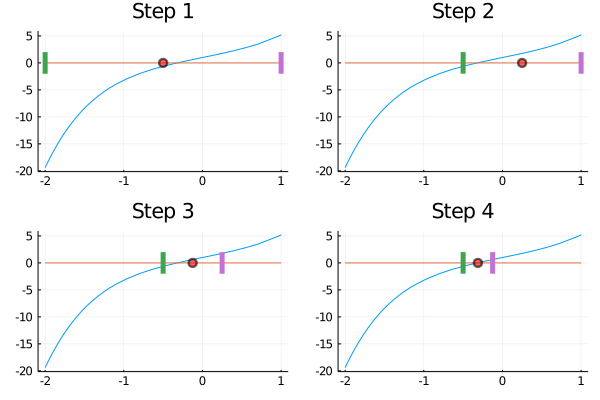
\includegraphics[scale=0.8]{Chap11NonlinearEquations/BisectionExample1.png}
    \caption[]{Evolution of the bracketing points $a$ and $b$ as well as the midpoint $c$ in the first four steps of the Bisection Algorithm for finding a root of $0.2x^5  + x^3 + 3x + 1=0$. It is very clear that the algorithm hones in on a root!
    } 
    \label{fig:BisectionExample1b}
    \end{figure}
    
    
     \begin{figure}[h!]
    \centering
    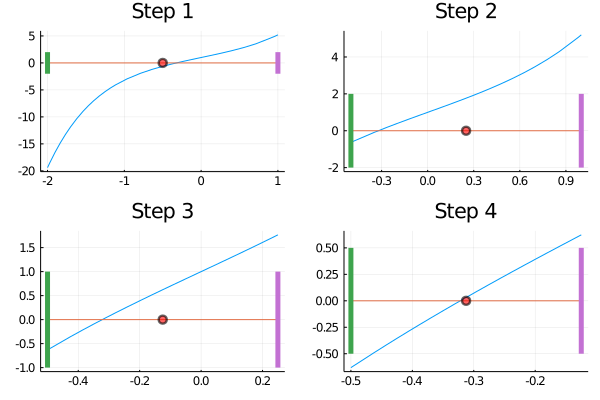
\includegraphics[scale=0.8]{Chap11NonlinearEquations/BisectionExample2.png}
    \caption[]{Zooms of the first four steps of the Bisection Algorithm for finding a root of $0.2x^5  + x^3 + 3x + 1=0$ that lies between $-1$ and $2$. Observe that as we zoom into the function at a point, it looks more and more like a straight line! 
    }
    \label{fig:BisectionExample1c}
    \end{figure}


%\vspace*{0.2cm}
\begin{tcolorbox}[sharp corners, colback=green!30, colframe=green!80!blue, title=\textbf{\large Linear Approximations of Functions can be Very Useful}]
Let's write the ``line'' in Step 4 of Fig.~\ref{fig:BisectionExample1c} in the form
$$y = y_c + m(x-c),$$
where $ y_c$ is the value of the line at $x=c$ and $m$ is the slope of the line. Using the data in \eqref{eq:BisectionExample1}, and the traditional notion of ``rise over run'' to define the slope, we obtain
%-0.5  -0.125  -0.63125  0.623041
\begin{align*}
        c&=-0.3125 \\
    y_c&=f(c)\approx 0.0313864 \\
        m&=\frac{f(b)-f(a)}{b-a}= \frac{0.623041 - (-0.63125)}{-0.125 - (-0.5 )}\approx 3.34478\\
\end{align*}
In Fig.~\ref{fig:LinearApproximationInspriedBisection}, we visually illustrate how good of a fit the ``line approximation'' 
$$y=0.0313864 + 3.34478(x+0.3125)=3.34478 x + 1.07663 $$
provides to the function. To show its utility,  
we set $y=0$ and solve for $x$. Doing so, we obtain
$$\boxed{ x^\ast = -0.321884\implies f(x^\ast)=0.00030674,}$$ 
an estimate of the root that it is much better than the value given by the Bisection Algorithm at Step 4! In fact, the Bisection Algorithm has to muddle along until its 12-th iteration to better this approximation of the root. \textbf{Issac Newton made this same observation back in 1669 and turned it into an algorithm for finding roots of equations.} 
\end{tcolorbox}


\begin{figure}[hbt!]
    \centering
    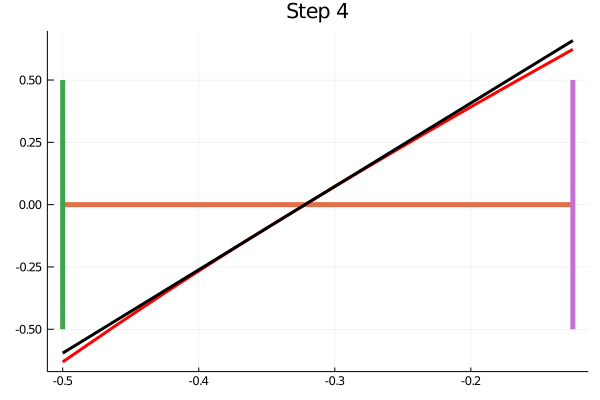
\includegraphics[scale=0.35]{Chap11NonlinearEquations/BisectionExample3LinearApproximationOfFunction.png}
    \caption[]{Linear Approximation (black) of $f(x)=0.2x^5  + x^3 + 3x + 1$ compared to the function itself (red). The linear approximation is very good in a sufficiently small region. 
    }
    \label{fig:LinearApproximationInspriedBisection}
    \end{figure}


%\vspace*{.05cm}

\begin{tcolorbox}[title=\textbf{\large Bisection Algorithm with Sanity Checks and Tolerance Included}]
The algorithm takes as input a generic function $f(x)$, bracketing points $a$ and $b$, and a tolerance value, ${\rm tol}$, for terminating the algorithm, where convergence is declared when $|f(c)| \le {\rm tol}$. The algorithm also terminates after $10^4$ iterations. 
The function returns the final values for $c$ and prints out $k$, the number of iterations it took to meet the convergence criteria.
    \begin{lstlisting}[language=Julia,style=mystyle]
function Bisection(f,a,b,tol)
    # First check the input data makes sense
    if !(a < b)
        println("a is not strictly less than b")
        return NaN
    end
    if !( f(a)*f(b) < 0)
        println("a and b fail the test provided by the Intermediate Value Theorem")
        return NaN
    end
    if tol < 1e-15
        println("tolerance is too tight")
        return NaN
    end
    c= (a+b)/2.0
    fc=f(c)
    k=0
#
# Ready to run the bisection algorithm 
# 
    while (abs(fc) > tol) & (k < 1e4) 
        if fc*f(a) < 0
            b=copy(c)
        else
            a=copy(c)
        end    
        c = (a+b)/2
        fc=f(c)
        k=k+1
    end
    println("Root is $c found at iteration $k")
    return c  
end
\end{lstlisting}
\end{tcolorbox}

\begin{lstlisting}[language=Julia,style=mystyle]
f(x)=0.2*x^5  + x^3 + 3*x + 1
a0=-2;b0=1
c=Bisection(f,a,b,1e-10)
@show f(c);
\end{lstlisting}
\textbf{Output}
\begin{verbatim}
Root is -0.3219763464294374 found at iteration 21
f(c) = -3.854006003223276e-11  
\end{verbatim}





\section{The Concept of a Derivative and Its Numerical Approximation}
\label{sec:NumericalDerivativesScalar}

\begin{figure}[hbt]%
\centering
\subfloat[]{%
    \label{fig:fitting}%
	\centering
  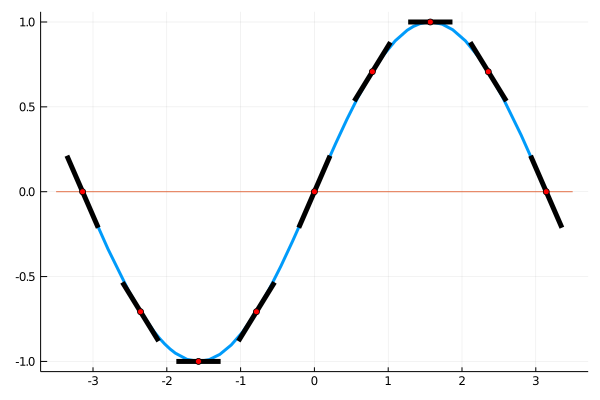
\includegraphics[width=0.48\columnwidth]{Chap11NonlinearEquations/DerivativeSine.png}
  }
  %\vspace{.2cm}
\subfloat[]{%
    \label{fig:ambiguity}%
	\centering
  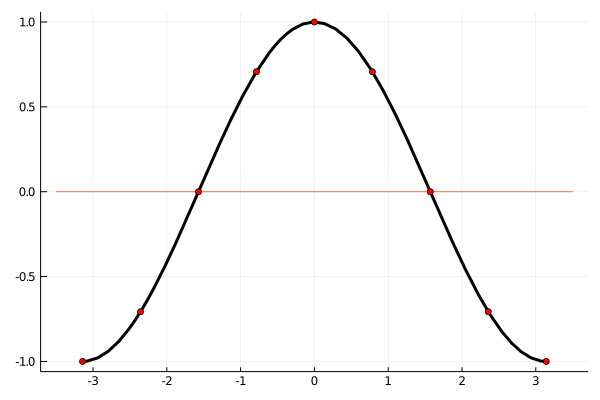
\includegraphics[width=0.48\columnwidth]{Chap11NonlinearEquations/DerivativeSine02.png}
  }
    \caption[]{(a) The line segments represent the local slope (``rise over run'') of $f(x)=\sin(x)$ at the points $[-\pi, -\frac{3 \pi}{4}, \ldots, \frac{3 \pi}{4}, \pi] $. Notice that each line segment is also a local linear approximation of the function. In a practical sense, what this means is that in a small region about a given point, we can replace the function with a local linear equivalent and then use linear techniques to analyze the function! In Calculus, the ``local slope of a function'' is called the derivative of the function. (b) The derivative of $f(x)$ is another function, denoted $\frac{df(x)}{dx}$. In Calculus, you will learn that $\frac{d}{dx}\sin(x) = \cos(x)$. Here, were are NOT using Calculus. We have computed the derivative numerically and plotted it! The maximum error in our numerical estimation of the derivative is less than $6.58 \times 10^{-6}$. }
    \label{fig:DerivativesExample01}
\end{figure}

Another concept that you will learn in Calculus is the \textbf{derivative of a function}. Geometrically, it is the slope of the function at a given point, say $x_0 \in \real$.  Note that if $x_1 \le x_0 < x_2$, then the ``rise'' of the function over the interval $(x_1, x_2)$ would be $d f(x_0): =f(x_2) - f(x_1)$, while the ``run'' would be $d x = x_2 - x_1$, and hence the ``slope'' would be 
$${\rm slope} := \frac{{\rm rise}}{{\rm run}}=\frac{d f (x_0)}{d x} = \frac{f(x_2) - f(x_1)}{x_2 - x_1}. $$


In Fig.~\ref{fig:DerivativesExample01}, we have attached short line segments with slopes corresponding to the derivative of the function $\sin(x)$ computed at a number of points. The hope is that this helps you grasp the geometric meaning of a derivative of a function at point as the ``local slope'' of the function at that point.
 We see that the ``local slope of the function'' varies with $x$. To tie the idea of ``slope equals rise over run'' to a given point, say $x_0$, we let $h \neq 0$ be a small number and then we define $x_1$ and $x_2$ in terms of $x_0$ and $h$, by $x_1=x_0$ and $x_2=x_0 + h$. This leads to
 \begin{equation}
\label{eq:forwardDifferenceV00}
    \frac{ d f(x_0) }{d x}= \frac{f(x_2) - f(x_1)}{x_2 - x_1} =\frac{f(x_0 + h) - f(x_0)}{(x_0+h) - x_0} = \frac{f(x_0 + h) - f(x_0)}{h}.
\end{equation}
In Calculus, one analyzes what happens in the limit when $h$ becomes very small, and in particular, one works hard to understand when the ratio in \eqref{eq:forwardDifferenceV00} approaches a well defined value as $h$ becomes smaller and smaller. While we'll explore this a bit in HW, it is beyond the scope of our effort here. 
\vspace*{.2cm}

\begin{tcolorbox}[title=\textbf{Numerical Approximations of a Derivative}]

We will adopt the traditional notation from Calculus for the limiting value in \eqref{eq:forwardDifferenceV00}, namely 
 \begin{equation}
\label{eq:forwardDifferenceV01}
    \frac{ df(x_0) }{d x}:= \lim_{h \to 0} \frac{f(x_0 + h) - f(x_0)}{h}.
\end{equation}

In practice, we will use ``small values'' for $h$ and never compute the exact limit. Hence, we have an \textbf{approximation for the derivative} at a point, namely
\begin{equation}
\label{eq:forwardDifference}
    \frac{df(x_0)}{dx}\approx \frac{f(x_0 + h) - f(x_0)}{h},
\end{equation}
which is called a \textbf{forward difference approximation to the derivative}. Note that we have replaced the informal term ``slope'' with the symbol for the derivative at a point, namely $\frac{df(x_0)}{dx}.$\\

You can also do a \textbf{backward difference approximation to the derivative},
\begin{equation}
\label{eq:backwardDifference}
   \frac{df(x_0)}{dx}\approx \frac{f(x_0) - f(x_0-  h)}{h},
\end{equation}
and a \textbf{symmetric difference approximation}, where you go both forward and backward from the point $x_0$,
\begin{equation}
\label{eq:symmetricDifference}
   \frac{df(x_0)}{dx}\approx \frac{f(x_0 + h)- f(x_0-  h)}{2 h}.
\end{equation}
The forward and backward difference approximations to the derivative are in fact exact for linear functions, while the symmetric difference approximation is \textit{exact} for quadratic polynomials. The symmetric difference is also sometimes called a \textbf{central difference}.\\

\textbf{If the derivative of $\mathbf{f(x)}$ at a point $\mathbf{x_0}$ exists, then for $\mathbf{h}$ sufficiently small, the forward difference, backward difference, and symmetric difference approximations to the derivative will always agree. If they provide different answers, then the limit in \eqref{eq:forwardDifferenceV01} does not exist and the function is said to be not differentiable.}

\end{tcolorbox}


\begin{lstlisting}[language=Julia,style=mystyle]
f(x)=sin.(x)
#
#
function SymmetricDifference(f,a,b)
    # f = generic function
    # does 100 equally spaced points from a to b
    # returns x and df/dx using Symmetric Differences
    if !(b > a)
        println("You need b > a")
    end
    N=100
    h=(b-a)/(10*N)
    x=LinRange(a,b,N) 
    x=collect(x)
    dfdx=0*x;
    for k=1:N
        dfdx[k]=(f(x[k]+h) - f(x[k]-h))/(2*h)
    end
    return dfdx, x
end
#
(dfdx,x)=SymmetricDifference(f,pi,-pi)
#
p1=plot(x, dfdx, legend=false,  linewidth=3, color=:black)
plot!(yzero,-3.5,3.5)
x0=[-pi -3*pi/4 -pi/2 -pi/4 0 pi/4 pi/2 3*pi/4 pi]'
df(x)=cos.(x) #Known from Calculus
              #included to make the plot look pretty??
y0=df(x0)
scatter!(x0,y0, color=:red)
plot(p1)
plot!(fmt = :png) 
\end{lstlisting}


\vspace*{0.2cm}
\begin{tcolorbox}[sharp corners, colback=green!30, colframe=green!80!blue, title=\textbf{\large Linear Approximation at a Point}]

The importance of being able to approximate a function in a region about a point by a linear function cannot be overstated. When studying the Bisection Method for finding roots, we noted that as we zoomed in on the function near the root, it looked more and more like a straight line. This property holds for all points $x_0$ at which a function is differentiable, that is, all points at which we can compute a derivative. \\

The linear function $y(x)$ that passes through the point $(x_0,y_0)$ with slope $m$ can be written as
$$y(x) = y_0 + m \left(x-x_0 \right). $$
We use this to define the \textbf{linear approximation of a function at a point} $\mathbf{x_0}$ by taking $y_0:=f(x_0)$ and $m:=\frac{df(x_0)}{dx}$. This gives us
\begin{equation}
    \label{eq:DefineLinearApproxScalarFunction}
   \boxed{\mathbf{ f(x)\approx f(x_0) + \frac{df(x_0)}{dx} \left(x-x_0 \right)}.}
\end{equation}
Figure~\ref{fig:LinearApproximationCubic} shows the linear approximation of a cubic about a point. For the record, in Calculus, this is called a First-order Taylor Expansion. You do not need to recall this terminology in ROB 101, but when you see it again in Calculus, you can say, yeah, I know why that is important! 

\end{tcolorbox}

\vspace*{.2cm} 

\begin{figure}[hbt!]
    \centering
    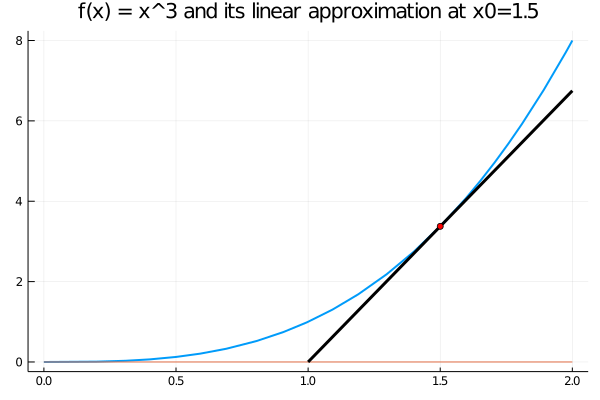
\includegraphics[width=0.7\columnwidth]{Chap11NonlinearEquations/LinearApproxCubic.png}
    \caption[]{The function $f(x)=x^3$ is plotted in cyan. The value of the function at the point $x_0=1.5$ is indicated in red. The line in black passing through $f(x_0)$ with slope $m=\frac{df(x_0)}{dx}$ satisfies $y(x):=f(x_0) + \frac{df(x_0)}{dx} \left( x - x_0 \right)$. The line is called the linear approximation of $f(x)$ at $x_0$. The linear approximation represents the function well in a sufficiently small region about $x_0$. This approximation can be done for any point $x_0$ at which the derivative exists. 
    }
    \label{fig:LinearApproximationCubic}
    \end{figure}

\textbf{Are all functions differentiable? No.} A minimum requirement for a function to be differentiable at a point is that the function be continuous at that point. Are there functions that are continuous and not differentiable? Yes, the classic example is $f(x) = |x|$, which is plotted in Fig.~\ref{fig:NotDifferentiable} and discussed in Example~\ref{ex:NonDifferentiableFunction}. 

\begin{figure}[hbt!]
    \centering
    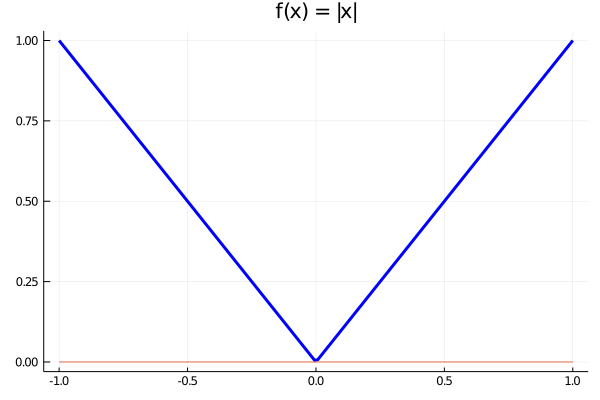
\includegraphics[width=0.7\columnwidth]{Chap11NonlinearEquations/NotDifferentiableAtOrigin.png}
    \caption[]{The function $f(x)=|x|$ is not differentiable at the origin ($x=0$). The slope of the function just to the left of the origin is $-1$, the slope just to the right of the origin is $+1$, and the slope at the origin is undefined. Everywhere else, the function is differentiable.
    }
    \label{fig:NotDifferentiable}
    \end{figure}


\begin{example}
\label{ex:NonDifferentiableFunction}
Explain why the function $f(x)=|x|$ is not differentiable at $x_0=0$. 
\end{example}

\textbf{Solution:} We compute the forward difference, backward difference, and symmetric difference approximations to the derivative at the point $x_0=0$ and see if we obtain similar answers or not. For this, we let $h>0$ be arbitrarily small. We note that then 
$$|h|=h, ~\text{and}~~ |-h| = - (-h) = h. $$


Proceeding, we compute 
\begin{align*}
    \textbf{forward difference  } ~& \frac{df(0)}{dx} \approx \frac{f(0+h) -f(0)}{h} = \frac{|h| - 0}{h} = \frac{h}{h} = \boxed{+1}\\
    \\
    \textbf{backward difference  }~ & \frac{df(0)}{dx} \approx \frac{f(0) -f(0-h)}{h} = \frac{0 - |-h|}{h} = \frac{-h}{h} = \boxed{-1}\\
    \\
    \textbf{symmetric difference  }~  &\frac{df(0)}{dx}   \approx \frac{f(0+h) -f(0-h)}{2h} = \frac{|h| - |-h|}{2h} = \frac{h-h}{2h} = \boxed{0}
\end{align*}

These three methods giving very different approximations to the ``slope'' at the origin is a strong hint that the function is not differentiable at the origin. What they are telling us is that by following different paths as we approach $x_0$, approaching $x_0$ from the left versus the right for example, gives different answers for the ``slope'' of the function at $x_0$. In Calculus, you'll learn that this means the function is not differentiable at $x_0$.


\Qed


\vspace*{0.5cm}

\section{Newton's Method for Scalar Problems}
\label{sec:newtonMethod}

We consider again the problem of finding roots of scalar equations $f(x)=0,$
where $f:\real \to \real.$ In the Bisection Algorithm, we only required that the function be continuous. The method we develop now uses the ``local slope information'' of a function, and hence requires that the function be differentiable, that is, that we can define $\frac{df(x)}{dx}$.\\

Let $x_k$ be our current approximation of a root of the function $f$. We write the linear approximation of $f$ about the point $x_k$ as
\begin{equation}
    \label{eq:NewtonMethod01}
    f(x) \approx f(x_k) + \frac{df(x_k)}{dx}\cdot (x - x_k).
\end{equation}
We want to chose $x_{k+1}$ so that $f(x_{k+1})=0$. Based on our linear approximation in \eqref{eq:NewtonMethod01}, we have that 
$$ f(x_{k+1}) \approx 0 \iff  0 =  f(x_k) + \frac{df(x_k)}{dx}\cdot (x_{k+1} - x_k).$$
If $\frac{df(x_k)}{dx}\neq 0$, we can solve for $x_{k+1}$, giving us 
\begin{align*}
\frac{df(x_k)}{dx} x_{k+1}& =   \frac{df(x_k)}{dx} x_k -f(x_k)\\
& \Downarrow \\
     x_{k+1} &=x_{k} -    {f(x_k)}\Big/{\frac{df(x_k)}{dx} }
\end{align*} 
For reasons that will become clear when we attempt a vector version of Newton's Algorithm, let's rewrite the division operation in the above formula as
$$ \boxed{    x_{k+1}=x_{k} - \left(   \frac{df(x_k)}{dx}\right)^{-1} f(x_k).}$$
The above equation is screaming for us to put it in a loop! One step of Newton's Method is shown in Fig.~\ref{fig:NewtonOneStep}.

\vspace*{0.5cm}
\begin{tcolorbox}[sharp corners, colback=green!30, colframe=green!80!blue,title=\textbf{Newton's Method}]

The iterative process
\begin{equation}
    \label{eq:NewtonMethod02}
x_{k+1}=x_{k} - \left(   \frac{df(x_k)}{dx}\right)^{-1} f(x_k)
\end{equation}
for finding a root of a nonlinear equation is called \textbf{Newton's Method} or \textbf{Newton's Algorithm}. Given the current approximation $x_k$ to a root of $f(x)$, Newton's Method corrects the approximation by the term  
$$-\left( \frac{df(x_k)}{dx}\right)^{-1} f(x_k) =  -{f(x_k)}\Big/{\frac{df(x_k)}{dx} }.$$  The validity of the next approximation $x_{k+1}$ rests upon: 
\begin{itemize}
    \item the function $f$ being differentiable;
    \item the derivative $\frac{df(x_k)}{dx}$ not vanishing at points generated by the algorithm in \eqref{eq:NewtonMethod02}; and
    \item \fbox{the linear equation \eqref{eq:NewtonMethod01} is a good approximation to the function.}
\end{itemize}
We boxed this last item because it is easy to overlook and is often a source of failure for the algorithm. Because \eqref{eq:NewtonMethod02} has ``total faith'' in \eqref{eq:NewtonMethod01} being a good approximation, it sometimes takes very big ``steps'' (meaning $x_{k+1}-x_k$ is large) when generating $x_{k+1}$ to zero the linear approximation in \eqref{eq:NewtonMethod01}. A safer update is to go only ``part way'' to the linear solution. This leads to the so-called \textbf{damped} or \textbf{modified Newton Method},
\begin{equation}
    \label{eq:NewtonMethodDamped}
\boxed{x_{k+1}=x_{k} - \epsilon \left(   \frac{df(x_k)}{dx}\right)^{-1} f(x_k)},
\end{equation}
where $0< \epsilon < 1$. A typical value may be $\epsilon=0.1$.\\

The standard way to ``ensure'' that Newton's Method generates points $x_k$ such that the linear equation \eqref{eq:NewtonMethod01} is a good approximation to $f(x_k)$ is to start the algorithm ``near'' a root. As you can imagine, this is easier said than done! Hence, the damped version of Newton's Algorithm is very useful in practice.

\end{tcolorbox}

\vspace*{.2cm}



\begin{figure}[hbt]%
    \centering
    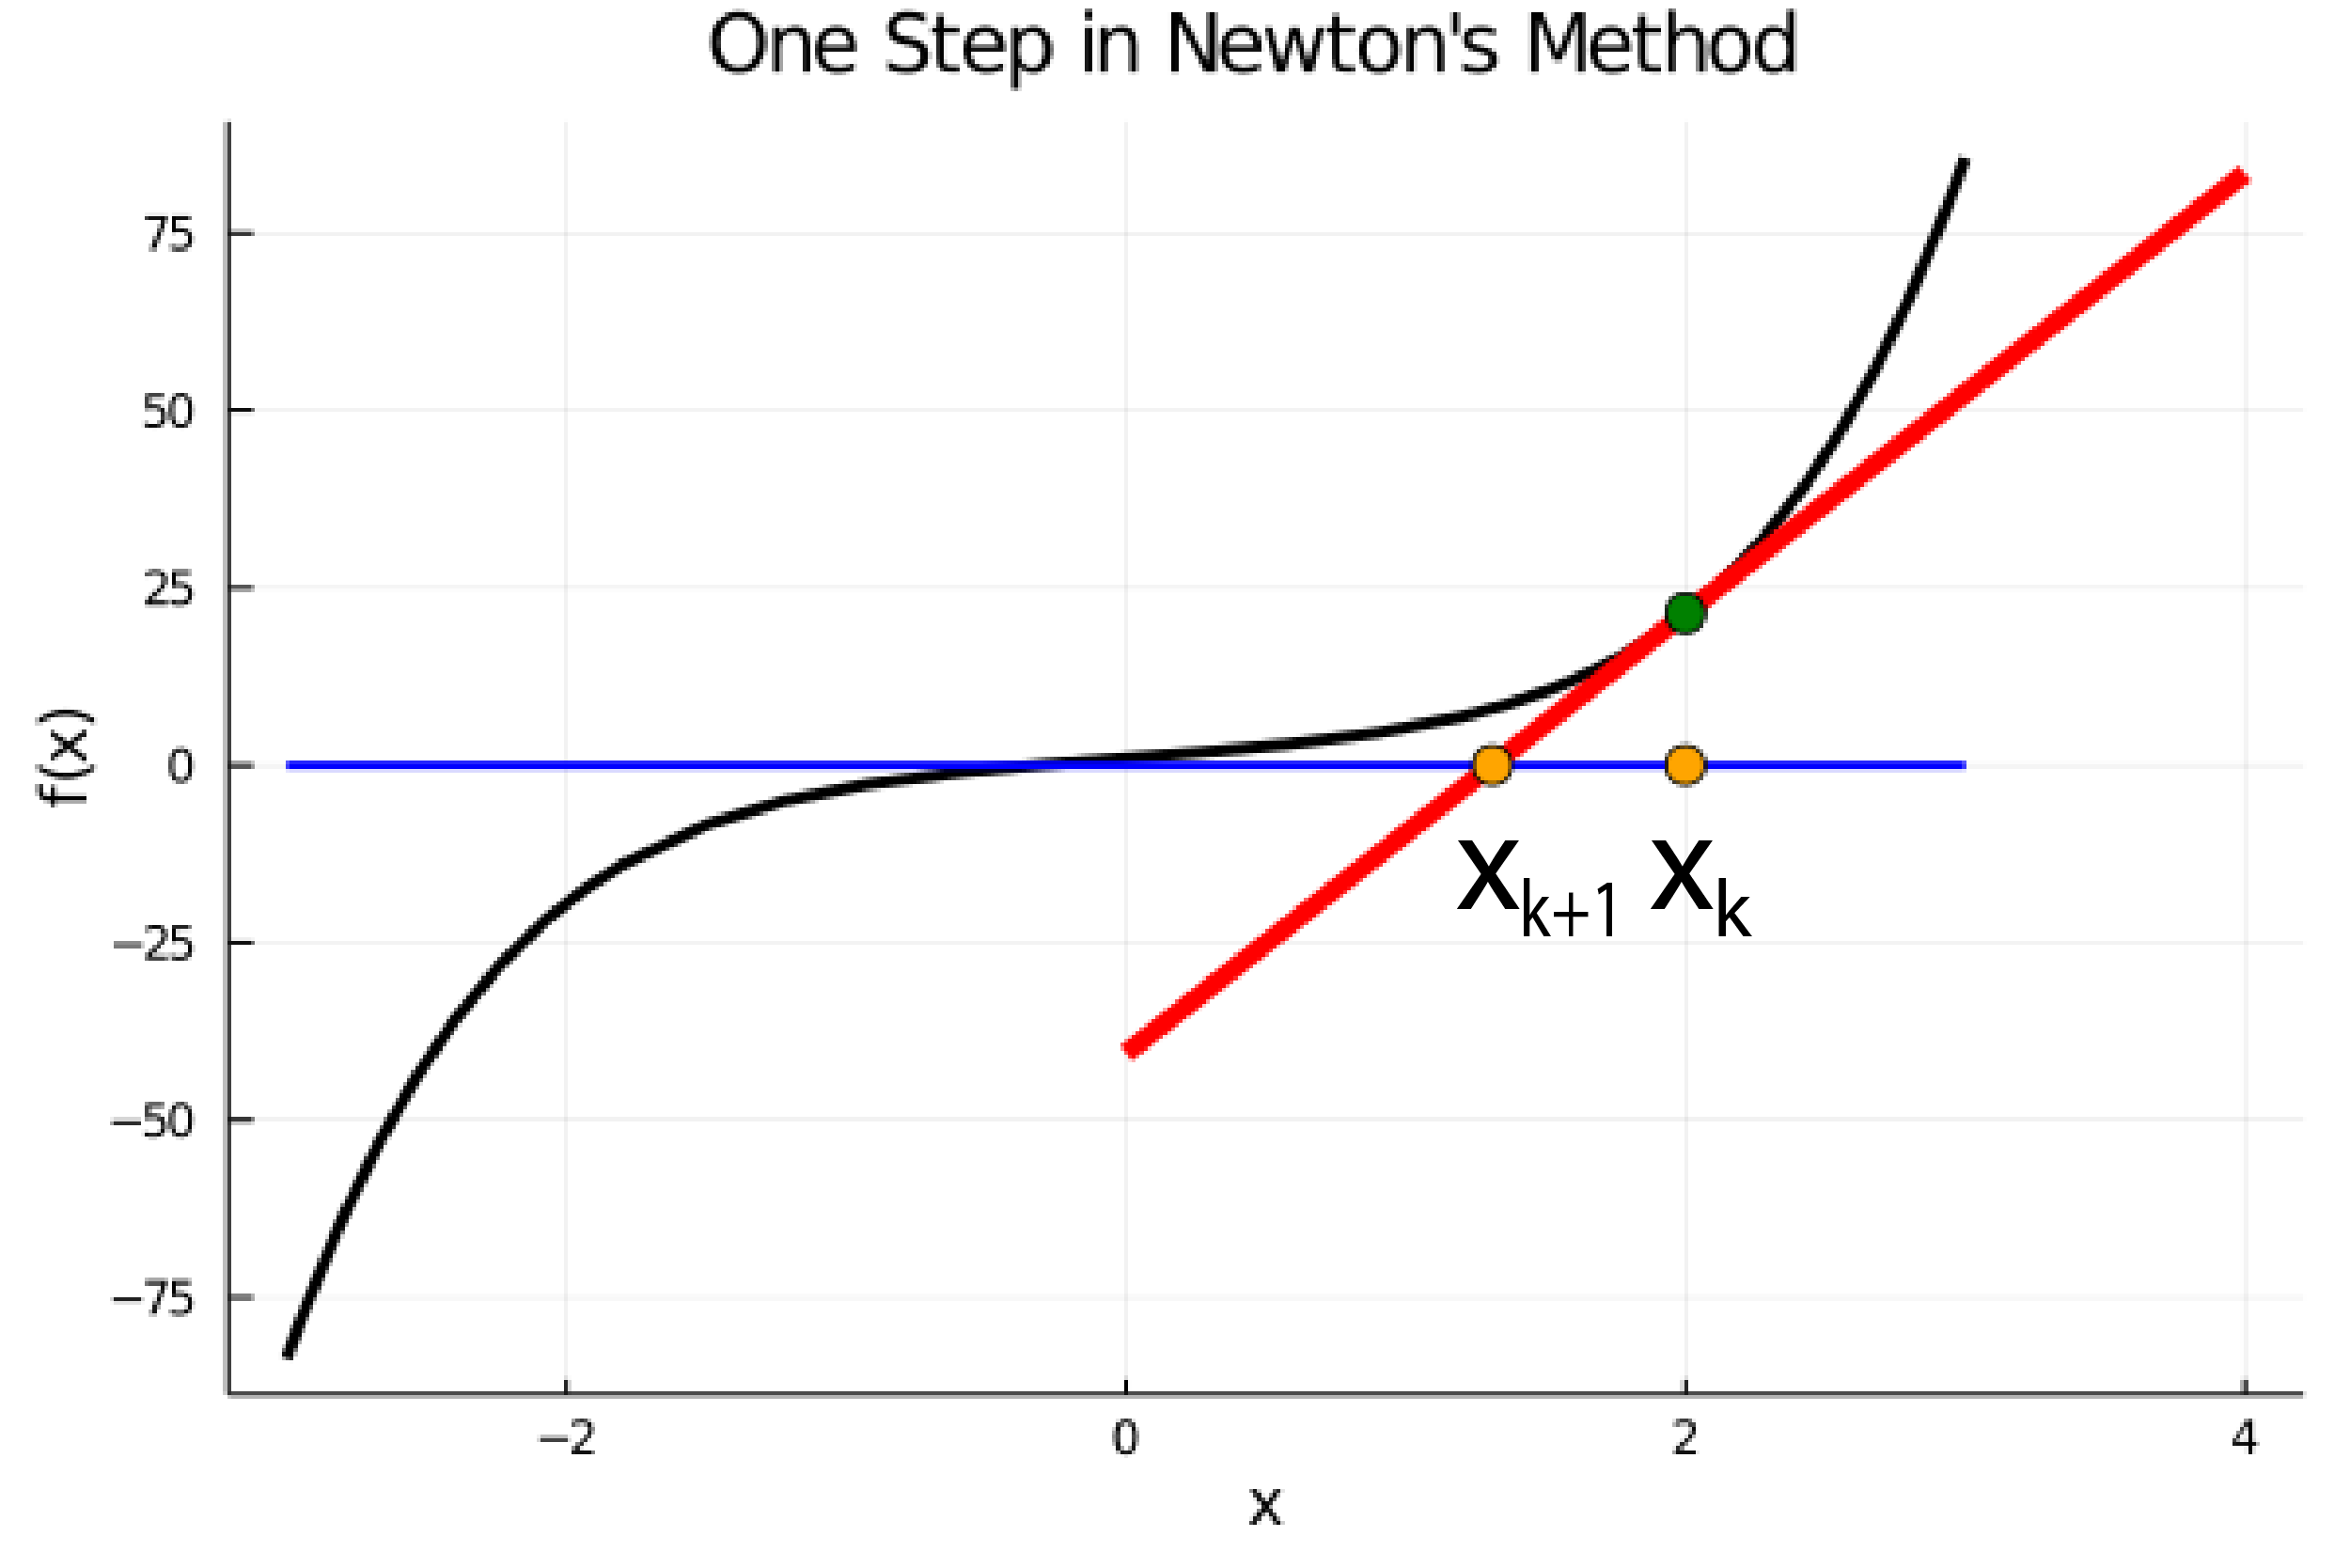
\includegraphics[trim=0 0 0 30,clip,height=0.4\textwidth]{Chap11NonlinearEquations/OneNewtonStepv02.png}
\caption[]{This figure demonstrates one step of Newton's Algorithm. At a point $x_k$, one uses the derivative to compute a linear approximation to the function. Solving for where the linear approximation (red line) crosses the $x$-axis gives the next value, $x_{k+1}$.}
\label{fig:NewtonOneStep}%
\end{figure}

\vspace*{.2cm}
\begin{tcolorbox}[title=\textbf{Visual Representation of Newton's Algorithm}]
Some of you are undoubtedly more visually wired than algebraically wired (did you know that was a thing?). Here are some potential visual sources:
\begin{itemize}
    \item Wikipedia \url{https://upload.wikimedia.org/wikipedia/commons/e/e0/NewtonIteration_Ani.gif} (The words in the legend are \textbf{function} and \textbf{tangent}.) You'll find additional textual information here as well \url{https://en.wikipedia.org/wiki/Newton%27s_method}
    \item Kahn Academy \url{https://www.youtube.com/watch?v=WuaI5G04Rcw}
    \item Christine Breiner, MIT Calculus I,  \url{https://www.youtube.com/watch?v=ER5B_YBFMJo}
\end{itemize}

\end{tcolorbox}


\vspace*{.2cm}

\begin{example}
\label{ex:NewtonMethod}
For the same function as treated in Example~\ref{ex:Bisection}, namely, $f(x)=0.2x^5  + x^3 + 3x + 1$, find a root using Newton's Algorithm. 

\end{example}

\textbf{Solution:} We apply the basic Newton's Method in \eqref{eq:NewtonMethod01} (that is, no damping), using each of the derivative methods given in \eqref{eq:forwardDifference}, 
\eqref{eq:backwardDifference}, and \eqref{eq:symmetricDifference}. We take $x_0=2$ and $h = 0.01$ for the approximate derivatives. We iterate until $|f(_k)| < 10^{-4}$ or the algorithm fails by $\left| \frac{df(x_k)}{dx} \right| < 10^{-4}$.\\

Using the \textbf{Symmetric Difference Approximation} for the derivative, Newton's Method converges in five steps
\begin{equation}
\begin{array}{rrrr}
{\bf x_k} & {\bf f(x_k) } &   {\bf \frac{df(x_k)}{dx}} &  {\bf k} \\
\\
2.0000 & 21.4000 & 31.2209 & 0.0000 \\
1.3146 & 8.0005 & 11.1709 & 1.0000 \\
0.5984 & 3.0247 & 4.2025 & 2.0000 \\
-0.1214 & 0.6341 & 3.0445 & 3.0000 \\
-0.3296 & -0.0255 & 3.3379 & 4.0000 \\
-0.3220 & -0.0001 & 3.3219 & 5.0000 \\
\end{array}
\end{equation}


Using the \textbf{Forward Difference Approximation} for the derivative, Newton's Method \textbf{fails} after 45 steps due to the estimated derivative vanishing
\begin{equation}
\begin{array}{rrrr}
{\bf x_k} & {\bf f(x_k) } &   {\bf \frac{df(x_k)}{dx}} &  {\bf k} \\
\\
2.0000 & 21.4000 & 31.2209 & 0.0000 \\
1.3146 & 8.0005 & -1328.6981 & 1.0000 \\
1.3206 & 8.0680 & 18.1162 & 2.0000 \\
0.8752 & 4.3989 & -360.9904 & 3.0000 \\
\vdots & \vdots &  \vdots &  \vdots  \\
5.4e+01 & 8.9e+07 & 7.6e+03  & 41.0000 \\
-1.2e+04 & -4.5e+19 & -4.5e+21 & 42.0000 \\
-1.2e+04 & -4.5e+19 & -8.1e+10 & 43.0000 \\
-5.5e+08 & -1.0e+43 & -1.0e+45 & 44.0000 \\
-5.5e+08 & -1.0e+43 & 0.0e+00 & 45.0000 \\
\end{array}
\end{equation}

Using the \textbf{Backward Difference Approximation} for the derivative, Newton's Method converges after 23 steps
\begin{equation}
\begin{array}{rrrr}
{\bf x_k} & {\bf f(x_k) } &   {\bf \frac{df(x_k)}{dx}} &  {\bf k} \\
\\
2.0000 & 21.4000 & 31.2209 & 0.0000 \\
1.3146 & 8.0005 & 1351.0399 & 1.0000 \\
1.3086 & 7.9346 & 17.5719 & 2.0000 \\
0.8571 & 4.2934 & 369.8273 & 3.0000 \\
0.8455 & 4.2272 & 12.2347 & 4.0000 \\
0.5000 & 2.6311 & 163.4044 & 5.0000 \\
0.4839 & 2.5702 & 9.8345 & 6.0000 \\
0.2225 & 1.6787 & 92.2938 & 7.0000 \\
0.2043 & 1.6216 & 8.8299 & 8.0000 \\
0.0207 & 1.0621 & 58.9551 & 9.0000 \\
0.0027 & 1.0080 & 8.4054 & 10.0000 \\
-0.1173 & 0.6466 & 39.1841 & 11.0000 \\
-0.1338 & 0.5963 & 8.0873 & 12.0000 \\
-0.2075 & 0.3685 & 25.9194 & 13.0000 \\
-0.2217 & 0.3239 & 7.6217 & 14.0000 \\
-0.2642 & 0.1887 & 16.7398 & 15.0000 \\
-0.2755 & 0.1524 & 6.8761 & 16.0000 \\
-0.2976 & 0.0803 & 10.4913 & 17.0000 \\
-0.3053 & 0.0552 & 5.8084 & 18.0000 \\
-0.3148 & 0.0238 & 6.4494 & 19.0000 \\
-0.3185 & 0.0116 & 4.5491 & 20.0000 \\
-0.3210 & 0.0031 & 4.1765 & 21.0000 \\
-0.3218 & 0.0006 & 3.5817 & 22.0000 \\
-0.3220 & 0.0000 & 3.3919 & 23.0000 \\
\end{array}
\end{equation}
\Qed

\begin{tcolorbox}[sharp corners, colback=green!30, colframe=green!80!blue,title=\textbf{Symmetric Difference Makes a Difference}]

In general, the symmetric difference is a better approximation to the true analytical derivative than are the forward and backward difference approximations. When used in Newton's Method, the big difference in performance of the three approximate derivative methods surprised us as well!\\

Why do people not use the symmetric difference all the time? Depending on the situation, you may have the value of $f(x_k)$ already at hand, in which case, to determine a forward or backward difference, you only need one additional function evaluation, namely, either $f(x_k + h)$ or $f(x_k - h)$, whereas with the symmetric difference, you must do both additional function evaluations. If $f$ is complicated to evaluate, that may bias you toward the computationally ``lighter'' methods. On the other hand, as we saw in our example with Newton's Algorithm, if you converge faster, you may still come out way ahead! \\

\textbf{The fact that the decision of which numerical differentiation method to use is not obvious and depends on the problem being solved is actually A GREAT THING: it keeps Engineers and Applied Mathematicians employed!} 

\end{tcolorbox}

% \vspace*{0.5cm}
\begin{remark} We redo the above example using the forward difference approximation of the derivative with $\epsilon = 0.9$. The results are that Newton's Method with damping converges, though very slowly.
$$
\begin{array}{rrrr}
{\bf x_k} & {\bf f(x_k) } &   {\bf \frac{df(x_k)}{dx}} &  {\bf k} \\
\\
2.0000 & 21.4000 & 31.2209 & 0.0000 \\
1.3831 & 8.8075 & -1246.7601 & 1.0000 \\
1.3895 & 8.8867 & 20.5359 & 2.0000 \\
1.0000 & 5.2000 & -361.6178 & 3.0000 \\
1.0129 & 5.2914 & 16.3261 & 4.0000 \\
0.7212 & 3.5779 & -166.4880 & 5.0000 \\
0.7406 & 3.6725 & 14.4315 & 6.0000 \\
0.5116 & 2.6755 & -95.8236 & 7.0000 \\
0.5367 & 2.7735 & 13.7664 & 8.0000 \\
0.3554 & 2.1121 & -62.7388 & 9.0000 \\
0.3857 & 2.2160 & 13.8764 & 10.0000 \\
\vdots & \vdots & \vdots & \vdots \\\
-0.3387 & -0.0558 & 6.8063 & 368.0000 \\
-0.3313 & -0.0311 & 5.8011 & 369.0000 \\
-0.3265 & -0.0150 & 4.9292 & 370.0000 \\
-0.3237 & -0.0059 & 4.2261 & 371.0000 \\
-0.3225 & -0.0017 & 3.7289 & 372.0000 \\
-0.3221 & -0.0003 & 3.4495 & 373.0000 \\
-0.3220 & -0.0000 & 3.3411 & 374.0000 \\
\end{array}
$$
    
\end{remark}


\section{Vector Valued Functions: Linear Approximations, Partial Derivatives, Jacobians, and the Gradient}
\label{sec:LinApproxPartialDerivJacobianGrad}

When developing Newtons' Method of root finding for functions $f:\real \to \real$, we started with the notion of a derivative being the local slope of a function at a point, and from there, we were led to the idea of locally approximating a nonlinear function by a line! Once we had the idea of a linear approximation of the function about a given point, Newton's Algorithm basically fell into our lap by solving for a root of the linear approximation. \\

For the vector case of functions $f:\real^m \to \real^n$, we'll turn things around a bit and start with the idea of a linear approximation of the function about a point and see how that leads us to the notion of a \textbf{partial derivative}. Once we have that concept down, the rest is book keeping, in other words, the rest is developing a nice matrix-vector formulation of a derivative of a function. It sounds harder than it is. Let's do it! \\

\textbf{Remark:} A more traditional approach that starts by introducing the notion of a partial derivative and, from there, builds the gradient, the Jacobian, and only then, introduces the idea of a linear approximation, maybe better for some readers. That path is followed in Chap.~\ref{sec:optionalread:GradjacobianLinear}.

\subsection{Linear Approximation about a Point: Take 1}

 Our goal is to generalize the idea of a linear approximation of a (nonlinear) function $f:\real^m \to \real^n $ at a point $x_0$. What we'll do is posit that the appropriate generalization should be 
 \begin{equation}
     \label{eq:PositLinearApprox}
     f(x) \approx f(x_0) + A ( x - x_0),
 \end{equation}
 where $A$ is an $n \times m$ matrix. We note that the dimensions make sense because $f(x_0)$ is $n \times 1$, $( x - x_0)$ is $m \times 1$, and therefore, $A ( x - x_0)$ is $n \times 1$. So far, so good.  \\
 
 Let's now figure out what the columns of $A$ need to be for \eqref{eq:PositLinearApprox} to hold of $x$ ``near'' $x_0$. We write $A=:\left[\begin{array}{cccc} a_1^{\rm col} & a_2^{\rm col} & \cdots & a_m^{\rm col}\end{array}\right],$ where  $a_j^{\rm col}$ is the $j$-th column of $A$. Further, let $\{ e_1, e_2, \ldots, e_m\}$ the canonical basis vectors for $\real^m$ (which we recall are the columns of the $m \times m$ identity matrix). We next recall that our ``sum over columns times rows'' method of matrix multiplication gives us that 
 $$ A e_j =  a_j^{\rm col}, $$ 
 which is true because, using ``Julia notation'', 
 $$(e_j)[i] = \begin{cases} 1 & i = j \\ 0 & \text{otherwise} \end{cases} $$
 implies that 
 $$ A e_j = \sum_{i=1}^m a_i^{\rm col}(e_j)[i] = a_j^{\rm col}.$$
 
 We let $x=x_0 + h e_j$ be a small perturbation about the nominal vlaue $x_0$. We note that $x=x_0 + h e_j$ \textbf{holds all components of $x$ constant and equal to $x_0$, except for the $j$-th component, which is perturbed by an amount $h$}. When  $h>0$ is sufficiently small, \eqref{eq:PositLinearApprox} gives us 
  \begin{equation}
     \label{eq:PositLinearApprox02}
     \begin{aligned}
          f(x_0 + h e_j) &= f(x_0) + A ( x_0 + h e_j - x_0)\\
          &\Downarrow \\
          f(x_0 + h e_j) &= f(x_0) + h A e_j \\
           &\Downarrow \\
          f(x_0 + h e_j) &= f(x_0) + h a_j^{\rm col}\\
                &\Downarrow \\
          f(x_0 + h e_j) - f(x_0)  &=  h a_j^{\rm col}\\
                          &\Downarrow \\
          \frac{f(x_0 + h e_j) - f(x_0)}{h}  &=  a_j^{\rm col}.
     \end{aligned}
 \end{equation}
 In other words, the $j$-th column of the matrix $A$ in \eqref{eq:PositLinearApprox} is given by
   \begin{equation}
     \label{eq:PositLinearApprox03}
     \boxed{
  a_j^{\rm col}= \frac{f(x_0 + h e_j) - f(x_0)}{h}, }
 \end{equation}
 which looks suspiciously like the forward difference approximation of a derivative. In fact, it looks like here we are ignoring all variables except the $j$-th one and computing a derivative of $f$ with respect to $x_j$. And indeed, that is exactly what we are doing! Calculus has a term for it, the \textbf{partial derivative of} $\mathbf{f(x)}$ with respect to $\mathbf{x_j}$, and it uses a cool symbol,
    \begin{equation}
     \label{eq:PartialDerivative}
     \boxed{
\frac{\partial f(x_0)}{\partial x_j}= \lim_{h \to 0} \frac{f(x_0 + h e_j) - f(x_0)}{h}.}
 \end{equation}
 The symbol $\partial$ is pronounced ``partial''. We'd better dig into this!
 
  \vspace*{0.2cm}
 


 
 \subsection{Partial Derivatives}
 
 \begin{tcolorbox}[title=\textbf{Partial Derivatives as Motivated by a Linear Approximation to a Function about a Point}]
If we let $\{e_1, e_2, \ldots, e_m \}$ be the natural basis vectors for $\real^m$, then we have three ways to \textbf{numerically approximate a partial derivative}, just as we did with a ``scalar'' derivative 
\begin{equation}
    \label{eq:partialDerivativesDifferenceApproximations}
    \frac{\partial f(x_0)}{\partial x_j}= \left\{ \begin{aligned}
        \frac{f(x_0+h e_j)-f(x_0)}{h}& ~~~ \text{forward difference approximation} \\
      \frac{f(x_0)-f(x_0-h e_j)}{h} &~~~  \text{backward difference approximation} \\
        \frac{f(x_0+h e_j)-f(x_0-h e_j)}{2h} & ~~~\text{symmetric difference approximation}.
    \end{aligned} \right.
    \end{equation}
\end{tcolorbox}
\vspace*{0.2cm}

 
 \begin{example}
 \label{ex:PartialDerivativesSymmericDifferences}
 %% \label{ex:JacobianBasedApproximation}
 For the function 
 \begin{equation}
 \label{eq:fR3ToR3}
 f(x_1,x_2,x_3):= 
 \left[
\begin{array}{c}
x_1 x_2 x_3  \\
\log(2+\cos(x_1)) + x_2^{x_1} \\
 \frac{x_1 x_3}{1+ x_2^2} \\
\end{array}
\right],
 \end{equation}
 compute the partial derivatives $\frac{\partial f(x_0)}{\partial x_1}$, $\frac{\partial f(x_0)}{\partial x_2}$, and $\frac{\partial f(x_0)}{\partial x_3}$ at the point 
 $$x_0 = \left[
\begin{array}{c}
\pi \\
1.0 \\
2.0 \\
\end{array}
\right].$$
\textbf{In the next example, we'll interpret the computed partial derivatives in terms of derivatives of scalar valued functions, which we intuitively understood as slopes of a function at a point.} 
  \end{example}
 
 \textbf{Solution A} We'll compute the partial derivatives in Julia, two different ways. We only need one of them to click for you. \\
 
 In the first solution, we write the function given in \eqref{eq:fR3ToR3} as $f(x)$, where $x=[x_1; x_2; x_3]$. We can then apply the numerical approximations in \eqref{eq:partialDerivativesDifferenceApproximations} directly. Because $f(x) \in \real^3$, the partial derivatives will also be vectors in $\real^3$. This follows from \eqref{eq:partialDerivativesDifferenceApproximations}, where each numerator is a  vector in $\real^3$, while the denominators are scalars.
 
 \begin{lstlisting}[language=Julia,style=mystyle]
x0=[pi;1.0;2.0]
# function defined in terms of x as a vector with components [x1; x2; x3].
function f(x)
    x1=x[1]
    x2=x[2]
    x3=x[3]
    f=[x1*x2*x3; log(2 + cos(x1) + x2^x1); (x1*x3)/(1+x2^2)]
    return f
end
h=0.001
Id=zeros(3,3)+I
e1=Id[:,1];e2=Id[:,2];e3=Id[:,3]
# Partial derivatives via symmetric differences
dfdx1=( f(x0+h*e1) - f(x0-h*e1) )/(2*h)
dfdx2=( f(x0+h*e2) - f(x0-h*e2) )/(2*h)
dfdx3=( f(x0+h*e3) - f(x0-h*e3) )/(2*h)

 \end{lstlisting}
Using the above code, we determine
  \begin{equation}
  \label{eq:PartialDerivativeAnswers}
\frac{\partial f(x_0)}{\partial x_1} = \left[
\begin{array}{c}
2.0 \\
0.0 \\
1.0 \\
\end{array}
\right], ~~\frac{\partial f(x_0)}{\partial x_2} = \left[
\begin{array}{r}
6.2832 \\
3.1416 \\
-3.1416 \\
\end{array}
\right],~~ \frac{\partial f(x_0)}{\partial x_3} = 
\left[
\begin{array}{c}
3.1416 \\
0.0000 \\
1.5708 \\
\end{array}
\right].
\end{equation}
\Qed

\vspace*{0.5cm}

\textbf{Solution B} In the second method, we express the function exactly as it is written in \eqref{eq:fR3ToR3}. We then have to recognize that
$$x_0 + h e_1 = (x_{01} +h, x_{02}, x_{03}),~ ~x_0 + h e_2 = (x_{01}, x_{02}+h, x_{03}),~ \text{and}~~ x_0 + h e_3 = (x_{01}, x_{02}, x_{03}+h).$$
The point is, in Mathematics,  we write a function that depends on several variables like this
$$f(x) = f(x_1, x_2, x_3) , $$
and never like this
\begin{equation}
    \label{eq:functionVectorized}
    f(x) = f(\left[
\begin{array}{c}
x_1 \\
x_2 \\
x_2 \\
\end{array}
\right] ).
\end{equation} 
However, when we program, it is often easier to work with a function as if it were written as in \eqref{eq:functionVectorized}, with $x$ a column vector; as an example,
$$f(x + h e_2) =   f(\left[
\begin{array}{c}
x_1 \\
x_2 \\
x_2 \\
\end{array}
\right] +\left[
\begin{array}{c}
0 \\
h \\
0 \\
\end{array}
\right] ) = f(x_1, x_2 + h, x_3). $$
You will learn quickly enough that it is easier to ``vectorize'' (that is, put operations in a loop) expressions such as $f(x + h e_2) = f(x + h Id[:, 2])$ than it is expressions such as$ f(x_1, x_2 + h, x_3)$, but we digress. 

\vspace*{0.2cm}

 \begin{lstlisting}[language=Julia,style=mystyle]
x0=[pi;1.0;2.0]
f(x1,x2,x3)=[x1*x2*x3; log(2 + cos(x1) + x2^x1); (x1*x3)/(1+x2^2)]
h=0.001

dfdx1=( f(pi+h,1.0,2.0) - f(pi-h,1,2) )/(2*h)  
dfdx2=( f(pi,1.0+h,2.0) - f(pi,1-h,2) )/(2*h)  
dfdx3=( f(pi,1.0,2.0+h) - f(pi,1,2-h) )/(2*h)
 \end{lstlisting}
 
The results match those in \eqref{eq:PartialDerivativeAnswers}. The code for the second solution looks simpler, doesn't it? But imagine writing that out if you have 25 variables! On the other hand, the code segment
\begin{lstlisting}[language=Julia,style=mystyle]
# As a loop
n=3
dfdx=Array{Float64,2}(undef,n,0)
for k =1:n
    dfdxk=( f(x0+h*Id[:,k]) - f(x0-h*Id[:,k]) )/(2*h)
    dfdx=[dfdx dfdxk]    
end
dfdx

3×3 Array{Float64,2}:
 2.0   6.28319  3.14159
 0.0   3.14159  0.0
 1.0  -3.14159  1.5708
\end{lstlisting}
is very easy to scale up! \textcolor{red}{\bf Vectors and matrices are really about careful bookkeeping. It's kind of sad to say it that way, but it's also kind of true.}
 \Qed
 
  \begin{example}
 \label{ex:PartialDerivativesSymmericDifferencesInterpretation}
For the function in Example~\ref{ex:PartialDerivativesSymmericDifferences}, interpret the components of its partial derivatives in terms of ``ordinary derivatives''.
 \end{example}
 
  \textbf{Solution} Let's quite arbitrarily focus on $x_2$. We define a function $g: \real \to \real^3$ by
  
  $$g(x_2) :=f(\pi,x_2,2) = \left[
\begin{array}{c}
\pi x_2 2 \\
\log(2+\cos(\pi)) + (x_2)^{\pi} \\
 \frac{\pi 2}{1+ (x_2)^2} \\
\end{array}
\right] = \left[
\begin{array}{c}
2 \pi  x_2 \\
(x_2)^{\pi} \\
 \frac{2 \pi }{1+ (x_2)^2} \\
\end{array}
\right],$$
where we have set $x_1 = \pi$ and $x_3=2$. Because the components of $g$ only depend on the single variable $x_2$, we can compute their ordinary derivatives about the point $x_{02} = 1$ using symmetric differences. We do so and determine that
$$ \frac{dg(x_{02})}{dx_2} \approx \frac{g(1+h)-g(1-h)}{2 h} = 
\left[
\begin{array}{r}
6.2832 \\
3.1416 \\
-3.1416 \\
\end{array}
\right]
.$$
We observe that $\frac{dg(x_{02})}{dx_2} = ~\frac{\partial f(x_0)}{\partial x_2}$. We also note that $g(x_2) $ being a column vector with three components does not really change anything: we are simply computing the slope of each component of $g$. 
  
  \Qed
  
  \vspace*{0.2cm}
  
\begin{tcolorbox}[title=\textbf{Partial Wisdom}]
Partial derivatives are simply ordinary derivatives that we perform one variable at time, while holding all other variables constant.\\
\begin{equation}
    \label{eq:PartialDerivativeForwardDifferenceWisdom}
    \begin{aligned}
          \frac{\partial f(x_0)}{\partial x_j} &\approx \frac{f(x_{01},\ldots, \mathbf{x_{0j} + h}, \ldots, x_{0m}) - f(x_{01}, \ldots,\mathbf{x_{0j}}, \ldots,  x_{0m})}{\mathbf{h}} \\
          &= \frac{f(x_{0} + h e_j) - f(x_0)}{\mathbf{h}}\\
          &= \frac{df(x_0 + x_j e_j)}{dx_j},
    \end{aligned}
\end{equation}
where the last expression is kind of awesome: it underlines that we have really fixed all of the components of $x$ EXCEPT for $x_j$ when we compute the partial derivative with respect to the $j$-th component of $x$; therefore, $\overline{f}(x_j):=f(x_0 + x_j e_j)$ is now a function of the scalar variable $x_j$ to which we can apply the ordinary derivative. The fact that $\overline{f}(x_j)\in \real^n$ means it has $n$-components instead of one has not really changed anything. For us, working with vectors or scalars, it's all the same.
\end{tcolorbox}   
  
  
\subsection{The Jacobian and Linear Approximation of a Function about a Point}

We now turn to functions $f:\real^m \to \real^n$. Based the compact notation introduced in \eqref{eq:partialDerivativesDifferenceApproximations}, we define the \textbf{Jacobian of a function} as
\begin{equation}
    \label{eq:DefJacobian}
    \frac{\partial f(x)}{\partial x}:=  \left[\begin{array}{cccc}
      \frac{\partial f(x)}{\partial x_1} & \frac{\partial f(x)}{\partial x_2} & \cdots & \frac{\partial f(x)}{\partial x_m}
    \end{array} \right]
\end{equation}
by packaging the column vectors $\frac{\partial f(x)}{\partial x_j}$ into a matrix. There is no mystery here as we discovered partial derivatives as the columns of a matrix back in \eqref{eq:PositLinearApprox03}. We need to keep in mind that, for each value of $x\in \real^m$, the compact and innocent looking object
$$ \frac{\partial f(x)}{\partial x} $$
is really an $n \times m$ matrix: once again, there are $m$ columns of the form $ \frac{\partial f(x)}{\partial x_j}$, and each column is an $n$-vector. When computing the Jacobian numerically, we typically build it up one column at a time as we did in Solution A to Example~\ref{ex:PartialDerivativesSymmericDifferences}. 

 \vspace*{.2cm}

Just for the record, we will write out $\frac{\partial f(x)}{\partial x}$ as an $n \times m$ matrix. We write
$$f(x) = \left[
\begin{array}{c}
f_1(x) \\
f_2(x)\\
\vdots \\
f_n(x)\\
\end{array}
\right] =  \left[ \begin{array}{c}
f_1(x_1, x_2, \dots, x_m) \\
f_2(x_1, x_2, \dots, x_m)\\
\vdots \\
f_n(x_1, x_2, \dots, x_m)\\
\end{array}
\right].$$
Writing out all of the entries in the $n \times m$ Jacobian matrix gives 
\begin{equation}
    \label{eq:VectorFunctions03}
    \frac{\partial f(x)}{\partial x} = \left[\begin{array}{cccc}
      \frac{\partial f_1(x)}{\partial x_1} & \frac{\partial f_1(x)}{\partial x_2} & \cdots & \frac{\partial f_1(x)}{\partial x_m} \medskip \\
      \frac{\partial f_2(x)}{\partial x_1} & \frac{\partial f_2(x)}{\partial x_2} & \cdots & \frac{\partial f_2(x)}{\partial x_m} \medskip \\
      \vdots & \vdots & \ddots & \vdots \medskip \\
      \frac{\partial f_n(x)}{\partial x_1} & \frac{\partial f_n(x)}{\partial x_2} & \cdots & \frac{\partial f_n(x)}{\partial x_m} 
    \end{array} \right].
\end{equation}
In other symbols, the $ij$ component of $\frac{\partial f(x)}{\partial x}$ is
$$ \left[ \frac{\partial f(x)}{\partial x}  \right]_{ij} = \frac{\partial f_i(x)}{\partial x_j}, $$
which is much more intimidating than \eqref{eq:DefJacobian}. \\

Perhaps it is better not to read any further? If you want to toss out the window all of the benefits of vector-matrix notation, you can compute each entry of the Jacobian matrix one by one, as in 
\begin{equation}
    \label{eq:VectorFunctions03B}
    \frac{\partial f_i(x)}{\partial x_j} \approx \frac{f_i(x_1, \ldots, x_j+h, \ldots, x_m) - f_i(x_1, \ldots, x_j-h, \ldots, x_m)}{2h}. 
    \end{equation}
In case you are wondering, your instructors almost never do this when doing real robotics! We use the ``vector version'' of the Jacobian where we compute each column of the matrix in a loop. However, for simple examples, such as $n=m=2$, the above very explicit scalar (means non-vector) calculations can be informative!

\vspace*{0.2cm}
\begin{tcolorbox}[title=\textbf{Linear Approximation at a Point for Functions of Vectors}]
The linear approximation of a (nonlinear) function $f:\real^m \to \real^n $ at a point $x_0$ is defined to be
 \begin{equation}
     \label{eq:DefineVectorLinearApprox}
     f(x) \approx f(x_0) + A ( x - x_0) = f(x_0) + \frac{\partial f(x_0)}{\partial x} ( x - x_0),
 \end{equation}
 where the $n \times m$ matrix $A$ is the Jacobian of $f$ at the point $x_0$. As we did previously, we note that the dimensions make sense because $f(x_0)$ is $n \times 1$, $( x - x_0)$ is $m \times 1$, and therefore, $\frac{\partial f(x_0)}{\partial x}  ( x - x_0)$ is $n \times 1$. 
\end{tcolorbox}


\begin{example}
 \label{ex:Jacobianbb}
 For the function 
 \begin{equation}
 \label{eq:fR3ToR3bb}
 f(x_1,x_2,x_3):= 
 \left[
\begin{array}{c}
x_1 x_2 x_3  \\
\log(2+\cos(x_1)) + x_2^{x_1} \\
 \frac{x_1 x_3}{1+ x_2^2} \\
\end{array}
\right],
 \end{equation}
 compute its Jacobian at the point 
 $$x_0 = \left[
\begin{array}{c}
\pi \\
1.0 \\
2.0 \\
\end{array}
\right]$$
and evaluate the ``accuracy'' of its linear approximation.

  \end{example}
 
 \textbf{Solution} From \eqref{eq:PartialDerivativeAnswers} in Example~\ref{ex:PartialDerivativesSymmericDifferences}, we have that
$$
\frac{\partial f(x_0)}{\partial x_1} = \left[
\begin{array}{c}
2.0 \\
0.0 \\
1.0 \\
\end{array}
\right], ~~\frac{\partial f(x_0)}{\partial x_2} = \left[
\begin{array}{r}
6.2832 \\
3.1416 \\
-3.1416 \\
\end{array}
\right],~~ \frac{\partial f(x_0)}{\partial x_3} = 
\left[
\begin{array}{c}
3.1416 \\
0.0000 \\
1.5708 \\
\end{array}
\right].
$$
Hence, packaging up the columns correctly gives the Jacobian at $x_0$,
$$ A:=\frac{\partial f(x_0)}{\partial x} = \left[
\begin{array}{rrr}2.0000 & 6.2832 & 3.1416 \\
0.0000 & 3.1416 & 0.0000 \\
1.0000 & -3.1416 & 1.5708 \\
\end{array}
\right],$$
and the linear approximation is
$$f(x) \approx f(x_0) + A (x-x_0) = \left[
\begin{array}{c}
6.2832 \\
1.0000 \\
3.1416 \\
\end{array}
\right] + \left[
\begin{array}{rrr}2.0000 & 6.2832 & 3.1416 \\
0.0000 & 3.1416 & 0.0000 \\
1.0000 & -3.1416 & 1.5708 \\
\end{array}
\right] \left[ \begin{array}{l}
x_1 - \pi \\
x_2 - 1.0 \\
x_3 - 2.0 \\
\end{array}
\right]. $$

\begin{lstlisting}[language=Julia,style=mystyle]
Jacf=[dfdx1 dfdx2 dfdx3]
\end{lstlisting}

One way to think about the question of assessing the quality of the linear approximation is to measure the error defined as
 $$e(x):= ||f(x)-f_{\rm lin}(x) ||,$$
 where $f_{\rm lin}(x):=f(x_0) + \frac{\partial f(x_0)}{\partial x} (x - x_0)$. We will seek to estimate the maximum value of $e(x)$ over a region containing the point $x_0$.
 Define 
 $$S(x_0):= \{x  \in \real^3 ~|~~~ |x_i-x_{0i} | \le d, i=1,2,3 \} $$
 and 
\begin{equation}
    \label{eq:MaxErrorLinApprox}
    {\rm Max~~ Error} := \max_{x\in S(x_0)} e(x) = \max_{x\in S(x_0)} ||f(x)-f_{\rm lin}(x) ||.
\end{equation}
For $d=0.25$, we used a ``random search'' routine and estimated that
$$ {\rm Max~~ Error}=0.12.$$
To put this into context, 
$$  \max_{x\in S(x_0)} ||f(x)|| = 8.47,$$
and thus the relative error is about $1.5\%.$
 \Qed
 
 \subsection{The Gradient and Linear Approximation of a Function about a Point}
 
 The \textbf{gradient} is simply the special name given to the Jacobian of a function $f:\real^m \to \real$, that is, for each $x \in \real^m$, $f(x)\in \real$ is a scalar. Along with its special name, it comes with a special symbol!
 
 \begin{tcolorbox}[title=\textbf{The Gradient and Linear Approximations}]
The \textbf{gradient} of $f:\real^m \to \real$ is simply the partial derivatives of $f$ with respect to $x_i$ arranged to form a \textbf{row vector},
\begin{equation}
    \label{eq:GradientDef}
    \nabla f(x_0):=\left[\begin{array}{cccc}
        \frac{\partial f(x_0)}{\partial x_1} &  \frac{\partial f(x_0)}{\partial x_2} & \cdots &  \frac{\partial f(x_0)}{\partial x_m} 
    \end{array} \right],
\end{equation}
which we can also call a $1 \times m$ matrix. The cool symbol $\nabla$ is usually pronounced as ``\textbf{grad}'' and one says ``\textbf{grad f}'' when speaking of $\nabla f$. \\

An important use of the gradient of a function of several variables is to form a \textbf{linear approximation of the function about a point}
\begin{equation}
    \label{eq:LinearModelofNLfunctionGrad}
      f(x) \approx f(x_0) + \nabla f(x_0) (x-x_0).
\end{equation}
Comparing this to \eqref{eq:PositLinearApprox}, we see that
$A= \nabla f(x_0)$,
a $1 \times m$ matrix. Expanding \eqref{eq:LinearModelofNLfunctionGrad} into its components gives
\begin{equation}
    \label{eq:LinearModelofNLfunctionGrad2}
    \begin{aligned}
      f(x) &\approx f(x_0) + \nabla f(x_0) (x-x_0)\\
      &=f(x_0) + \underbrace{\left[\begin{array}{cccc}
        \frac{\partial f(x_0)}{\partial x_1} &  \frac{\partial f(x_0)}{\partial x_2} & \cdots &  \frac{\partial f(x_0)}{\partial x_m} 
    \end{array} \right]}_{A} \cdot \underbrace{\left[\begin{array}{c}
        x_1-x_{01} \\
        x_2-x_{02} \\
        \vdots \\
        x_m-x_{0m}
    \end{array} \right]}_{(x-x_0)} \\
     &= f(x_0) + \sum_{i=1}^m  \frac{\partial f(x_0)}{\partial x_i} (x_i-x_{0i}).
      \end{aligned}
\end{equation}
The linear approximation in \eqref{eq:LinearModelofNLfunctionGrad2} looks just like our linear approximation for functions of a single variable $x$, namely $f(x) \approx f(x_0) + \frac{df(x_0)}{ dx} (x-x_0)$, where $a= \frac{df(x_0)}{ dx}$ is $1 \times 1.$

\end{tcolorbox}

\vspace*{.2cm}

\begin{figure}[hbt!]
    \centering
    \subfloat[]{%
	\centering
    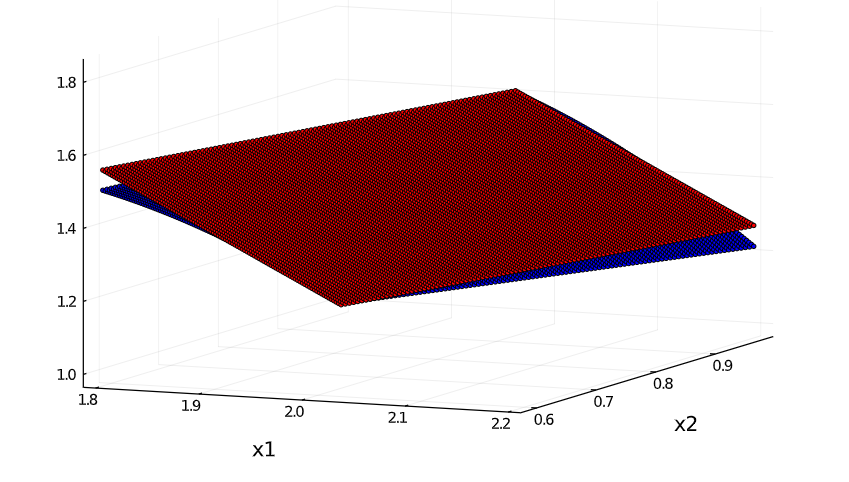
\includegraphics[width=0.48\columnwidth]{Chap11NonlinearEquations/VectorLinearApprox.png}
    }
      %\vspace{.2cm}
\subfloat[]{%
	\centering
  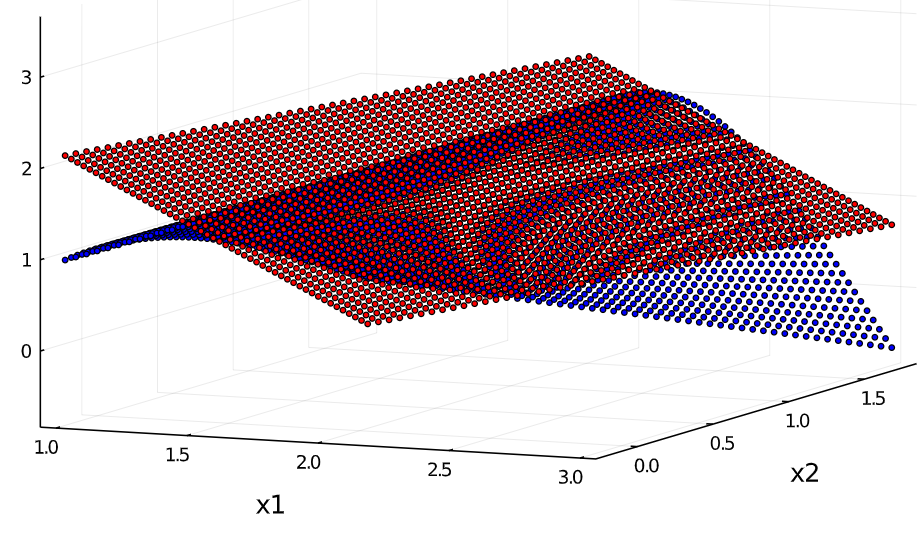
\includegraphics[width=0.48\columnwidth]{Chap11NonlinearEquations/LinearApproximationMoreCurvature.png}
  }
    \caption[]{(a) Close up view. (b) A more global view. The function $f(x_1, x_2) = x_1 \cos(x_2)$ is plotted in blue, while in red is shown its linear approximation about the point $x_0=[2~~\pi/4]^\top$, that is,  $f_{\rm lin}(x) :=f(x_0) + \nabla f(x_0) (x-x_0)$. This approximation can be done for any point $x_0$ at which the partial derivatives exists. In Calculus, the red plane is also called the \textbf{tangent plane at} $\mathbf{x_0}$. These linear approximations accurately represent the nonlinear function in a small enough region about a given point, allowing us to use our Linear Algebra skills. 
    }
    \label{fig:VectorLinearApprox}
    \end{figure}

\vspace*{.2cm}

\begin{example} 
\label{ex:GradientPartialDerivative} 
Compute (approximately) the gradient of $f:\real^2 \to \real$, for $f(x_1, x_2) = x_1 \cos(x_2)$ and $x_0=[2~~\pi/4]^\top$.
\end{example}

\textbf{Solution:} Let's get the formulas for a general $h>0$ and then we'll build a Table comparing the results for several values of $h$. For the partial derivative with respect to $x_1$, we perturb $x_1$ abut $2$ while holding $x_2$ constant and equal to $\pi/4$. This gives
\begin{align*}
    \frac{\partial f(x_0)}{\partial x_1}& \approx\frac{f(2+h,\pi/4) - f(2-h,\pi/4)}{2h} \medskip \\
    &= \frac{ (2+h) \cos(\pi/4) - (2-h) \cos(\pi/4)}{2h} \medskip \\
        &= \frac{ 2h\cos(\pi/4)}{2h} \medskip \\
    &= \cos(\pi/4) = \frac{\sqrt{2}}{2},
\end{align*}
which is independent of $h$ and hence there is nothing more to compute. For the next partial derivative, we perturb $x_2$ about $\pi/4$ while holding $x_1$ constant and equal to $2$. This gives
\begin{equation}
\begin{aligned}
    \frac{\partial f(x_0)}{\partial x_2}&\approx \frac{f(2,\pi/4+h) - f(2,\pi/4-h)}{2h} \medskip \\
    &= \frac{ 2 \cos(\pi/4+h) - 2 \cos(\pi/4-h)}{2h},
\end{aligned}
\end{equation}
which, though we could simply it with some trigonometric identities, we'll stop here and turn to Julia. Doing so, leads to the following results
\begin{equation}
\begin{array}{ll}
\frac{f(2,\pi/4+h) - f(2,\pi/4-h)}{2h} & ~~~h \\
\\
-1.41421356001592 & 0.0001 \\
-1.414213326670799 & 0.001 \\
-1.4141899922649026 & 0.01 \\
-1.4118577179998826 & 0.1 \\
-1.4048043101898116 & 0.2 \\
-1.3768017528243548 & 0.4 \\
\end{array}
\end{equation}
The true answer is 
$$ \frac{\partial f(2, \pi/4)}{\partial x_2} = -\sqrt{2} \approx -1.4142135623730951 $$
\Qed

\vspace*{0.2cm}

\begin{example} 
\label{ex:Gradient} 
Compute a linear approximation of $f(x_1, x_2) = x_1 \cos(x_2)$ at the point $x_0=[2~~\pi/4]^\top$.
\end{example}

\textbf{Solution:} We know both of the partial derivatives of $f$ at the point $x_0=[2~~\pi/4]^\top$. Hence, we have
\begin{equation}
    \label{eq:gradientExample}
    \begin{aligned}
  f(x) &\approx f(x_0) + \nabla f(x_0) (x-x_0)\\
    &= f(x_0)  + \left[\begin{array}{cc}
        \frac{\partial f(x_0)}{\partial x_1} &  \frac{\partial f(x_0)}{\partial x_2}
    \end{array} \right]  \left[\begin{array}{c}
        x_1-x_{01} \\
        x_2-x_{02} \\
           \end{array} \right]\\
    &= 2 \cos(\pi/4) + \left[
    \begin{array}{cc}
        \frac{\sqrt{2}}{2} & -\sqrt{2}\end{array} \right] \left[\begin{array}{c}
        x_1-2 \\
        x_2-\pi/4 \\
           \end{array} \right]
    \end{aligned}
\end{equation}

Figure~\ref{fig:VectorLinearApprox} compares the linear approximation to the nonlinear function in a region about $x_0$. 
\Qed

 
 
 
\begin{tcolorbox}[sharp corners, colback=green!30, colframe=green!80!blue,title=\textbf{Knowledge is Power}]
For root finding, an accuracy of a few percent is probably good enough. That said, \textbf{learning how to compute the partial derivatives analytically will make your code faster and will eliminate the question of how to choose the small perturbation parameter $h>0$.}
\end{tcolorbox}
  
  
\subsection{Summary on Partial Derivatives}
\label{sec:optional:CompactDerivativeNotation}

\begin{tcolorbox}[sharp corners, colback=green!30, colframe=green!80!blue,title={\textbf{From slopes of lines}$\to$\textbf{slopes of functions at points}~$\mathbf{\to \frac{df(x_0)}{dx} \to \nabla f(x_0) \to \frac{\partial f(x_0)}{\partial x}}$}]
Derivatives, gradients, and Jacobians are all generalizations of the notion of the slope  of a line being its ``rise over run''. The derivative of a function $f:\real \to \real$ at a point $x_0$ is the ``local'' slope of the function at that point. We compute it by ``rise over run'', where, for example
\begin{equation}
    \label{eq:SummaryDerivative}
 \text{\rm slope} = \frac{f(x_0+h)-f(x_0)}{h} \xrightarrow[h>0~\text{small}]{} \frac{df(x_0)}{dx},
\end{equation}
and to make it local, we take $h>0$ small. The gradient recognizes that a function $f:\real^m \to \real$ has a local slope in the $x_1$-direction, the $x_2$-direction, all the way up to the $x_m$-direction. If we let $\{e_1, e_2, \ldots, e_m \}$ be the natural basis vectors for $\real^m$, then we compute each component of the gradient by 
\begin{equation}
    \label{eq:SummaryGradient01}
    \text{\rm slope}_j = \frac{f(x_0+h e_j)-f(x_0)}{h}  \xrightarrow[h>0~\text{small}]{} \frac{\partial f(x_0)}{\partial x_j}, 
    \end{equation}
and we assemble the gradient by 
\begin{equation}
    \label{eq:SummaryGradient02}
\nabla f(x_0):= \left[\begin{array}{cccc} \frac{\partial f(x_0)}{\partial x_1} & \frac{\partial f(x_0)}{\partial x_2} & \cdots & \frac{\partial f(x_0)}{\partial x_m}
\end{array} \right]. 
\end{equation}
Finally, for $f:\real^m \to \real^n$, each of the $n$ components of $f(x)$ has a local slope with respect to each component of $x$. The bookkeeping is easiest if we leave $f(x)$ as a vector and write the Jacobian so that it \textbf{looks just like} the gradient,  
\begin{equation}
    \label{eq:SummaryJacobian01}
    \frac{ \partial f(x_0) }{\partial x}:= \left[\begin{array}{cccc} \frac{\partial f(x_0)}{\partial x_1} & \frac{\partial f(x_0)}{\partial x_2} & \cdots & \frac{\partial f(x_0)}{\partial x_m}
\end{array} \right],  
\end{equation}
but now, because $f(x)$ is an $n$-vector, we have 
\begin{equation}
    \label{eq:SummaryJacobian02}
    \left[\begin{array}{c}  \text{\rm slope}_{1j}\\ \vdots \\ \text{\rm slope}_{ij} \\ \vdots \\ \text{\rm slope}_{nj} \end{array}  \right] = \frac{f(x_0+h e_j)-f(x_0)}{h}  \xrightarrow[h>0~\text{small}]{} \frac{\partial f(x_0)}{\partial x_j}. 
\end{equation}
\end{tcolorbox}

\begin{tcolorbox}[title=\textbf{Compact Way to Numerically Approximate the Jacobian}]
If we let $\{e_1, e_2, \ldots, e_m \}$ be the natural basis vectors for $\real^m$, then vector notation allows us to compute each column of the Jacobian by 
\begin{equation}
    \label{eq:SummaryGradient01A}
    \frac{\partial f(x_0)}{\partial x_j} = \frac{f(x_0+h e_j)-f(x_0)}{h}.
    \end{equation}
    Typically, this is easier to program up than \eqref{eq:VectorFunctions03B}. But of course, your experience may vary! For a symmetric difference, we'd use
    \begin{equation}
    \label{eq:SummaryGradient01B}
    \frac{\partial f(x_0)}{\partial x_j} = \frac{f(x_0+h e_j)-f(x_0- h e_j)}{2h}.
    \end{equation}
\end{tcolorbox}



\section{Newton-Raphson for Vector Functions}
\label{sec:Newtonraphson}

We consider functions $f:\real^n \to \real^n$ and seek a root $f(x_0)=0$. Note that the domain and range are both $\real^n$ and thus this is the nonlinear equivalent of solving a square linear equation $Ax-b=0$. We recall that $\det(A)\neq 0$ was our magic condition for the existence and uniqueness of solutions to $Ax-b=0$. \\

The \textbf{Newton-Raphson} Algorithm is precisely a vector version of Newton's Algorithm. Let $x_k$ be our current approximation of a root of the function $f$. We write the linear approximation of $f$ about the point $x_k$ as
\begin{equation}
    \label{eq:NewtonMethodVector01}
    f(x) \approx f(x_k) + \frac{\partial f(x_k)}{\partial x}\cdot (x - x_k).
\end{equation}
We want to chose $x_{k+1}$ so that $f(x_{k+1})=0$. Based on our linear approximation in \eqref{eq:NewtonMethodVector01}, we have that 
\begin{equation}
    \label{eq:BasicNewtonRaphson}
     f(x_{k+1}) \approx 0 \iff  0  \approx f(x_k) + \frac{\partial f(x_k)}{\partial x}\cdot (x_{k+1} - x_k).
\end{equation}
If $\det\left(\frac{\partial f(x_k)}{\partial x} \right)\neq 0$  we could naively solve for $x_{k+1}$, giving us
$$ \boxed{    x_{k+1}=x_{k} - \left(   \frac{\partial f(x_k)}{\partial x}\right)^{-1} f(x_k).}$$
By now, you know that we advise against blindly computing inverses of matrices unless you really need that matrix inverse. In our case, what we really want is $x_{k+1}$, and because we know to avoid computing unnecessary matrix inverses, we'll write the algorithm down in a different way. 
As in the scalar case, the equation is screaming for us to put it in a loop!

\vspace*{0.2cm}
\begin{tcolorbox}[sharp corners, colback=green!30, colframe=green!80!blue,title=\textbf{Newton-Raphson Algorithm}]
Based on \eqref{eq:BasicNewtonRaphson}, we define\footnote{Note that $\Delta x_k = x_{k+1}-x_k$.} $x_{k+1}:= x_k + \Delta x_k$, where $ \Delta x_k$ is our update to $x_k$. We can then break the algorithm into two steps,
\begin{align}
\label{eq:NewtonRaphsonStep1}
\left(\frac{\partial f(x_k)}{\partial x} \right) \Delta x_{k} &= - f(x_k) \hspace*{0.58cm}(\text{solve for}~~\Delta x_k)  \\
\label{eq:NewtonRaphsonStep2}
x_{k+1}&= x_k + \Delta x_{k}~~(\text{use~~} \Delta x_k ~~\text{to update our estimate of the root}).
\end{align}
While for toy problems, we can use the matrix inverse to solve \eqref{eq:NewtonRaphsonStep1} for $\Delta x_{k}$, for larger problems, we recommend using an LU Factorization or a QR Factorization. Once \eqref{eq:NewtonRaphsonStep1}  has been solved, $x_{k+1}$ is updated in \eqref{eq:NewtonRaphsonStep2} and the process repeats.\\

A \textbf{damped Newton-Raphson Algorithm} is obtained by replacing \eqref{eq:NewtonRaphsonStep2} with   
\begin{equation}
    \label{eq:NewtonRaphsonStep3}
x_{k+1}= x_k + \epsilon \Delta x_{k},
\end{equation}
for some $\epsilon >0$.
 The validity of the Newton-Raphson Algorithm rests upon: 
\begin{itemize}
    \item the function $f$ being differentiable;
    \item the Jacobian $\frac{\partial f(x_k)}{ \partial x}$ having a non-zero determinant at points generated by \eqref{eq:NewtonRaphsonStep1} and \eqref{eq:NewtonRaphsonStep2}; and
    \item \fbox{the linear equation $f_{\rm lin}(x) = f(x_k) + \frac{\partial f(x_k)}{ \partial x} (x - x_k) $ being a good approximation to the function.}
\end{itemize}

\end{tcolorbox}


      
    

\begin{example}
\label{ex:NewtonRaphson}
Find a root of $F:\real^4 \to \real^4$ near $x_0=\left[\begin{array}{cccc} -2.0 & 3.0 & \pi &-1.0\end{array} \right]$ for
$$
F(x)=\left[\begin{array}{c}
   x_1 + 2 x_2 - x_1 (x_1 + 4 x_2) - x_2 (4 x_1 + 10 x_2) + 3 \medskip \\
 3 x_1 + 4 x_2 - x_1 (x_1 + 4 x_2) - x_2 (4 x_1 + 10 x_2) + 4  \medskip\\
                                0.5 \cos(x_1) + x_3 -\left( \sin(x_3) \right)^7  \medskip\\
                              -  2(x_2)^2  \sin(x_1) + (x_4)^3
\end{array} \right].
$$

\end{example}

\textbf{Solution:} We programmed up \eqref{eq:NewtonRaphsonStep1} and \eqref{eq:NewtonRaphsonStep2} in Julia and used a symmetric difference approximation for the derivatives, with $h=0.1$. Below are the first five results from the algorithm:
$$
x_k = \left[
\begin{array}{rrrrrr}
k=0~~ & k=1~~ & k=2 ~~& k=3~~ & k=4~~& k=5~~ \medskip \\
-2.0000 & -3.0435 & -2.4233 & -2.2702 & -2.2596 & -2.2596 \\
3.0000 & 2.5435 & 1.9233 & 1.7702 & 1.7596 & 1.7596 \\
3.1416 & 0.6817 & 0.4104 & 0.3251 & 0.3181 & 0.3181 \\
-1.0000 & -1.8580 & -2.0710 & -1.7652 & -1.6884 & -1.6846 
\end{array}
\right]
$$
and
$$
f(x_k) = 
\left[
\begin{array}{rrrrrr}
k=0~~ & k=1~~ & k=2 ~~& k=3~~ & k=4~~& k=5~~ \medskip\\
-39.0000 & -6.9839 & -1.1539 & -0.0703 & -0.0003 & -0.0000 \\
-36.0000 & -6.9839 & -1.1539 & -0.0703 & -0.0003 & -0.0000 \\
2.9335 & 0.1447 & 0.0323 & 0.0028 & 0.0000 & -0.0000 \\
15.3674 & -5.1471 & -4.0134 & -0.7044 & -0.0321 & -0.0001
\end{array}
\right].
$$
By iteration five, we have a good approximation of a root because $||f(x_5)|| \approx 10^{-4}$.
We also provide the Jacobians at the initial and final steps,
$$
 \frac{\partial f(x_0)}{\partial x}=\left[
\begin{array}{rrrr}
-19.0000 & -42.0000 & 0.0000 & 0.0000 \\
-17.0000 & -40.0000 & 0.0000 & 0.0000 \\
0.4539 & 0.0000 & 1.0000 & 0.0000 \\
7.4782 & 10.9116 & 0.0000 & 3.0100 \\
\end{array}
\right] \text{~~and~~}  \frac{\partial f(x_5)}{\partial x} = 
\left[
\begin{array}{rrrr}
-8.5577 & -15.1155 & 0.0000 & 0.0000 \\
-6.5577 & -13.1155 & 0.0000 & 0.0000 \\
0.3854 & 0.0000 & 0.9910 & 0.0000 \\
3.9296 & 5.4337 & 0.0000 & 8.5616 \\
\end{array}
\right]
$$
so that it is clear that as $x_k$ evolves, so does the Jacobian of $f$ at $x_k$.
\Qed

\section{(Optional Read): From the Gradient or Jacobian of a Function to its Linear Approximation}
\label{sec:optionalread:GradjacobianLinear}

\textbf{This covers the same material as in Chap.~\ref{sec:LinApproxPartialDerivJacobianGrad}, but in reverse order. Some may find it more digestible.}\\


Consider a function $f:\real^m \to \real^n$. We seek a means to build a linear approximation of the function near a given point $x_0 \in \real^m$. When $m=n=1$, we were able to approximate a function by 
$$ f(x) \approx f(x_0) + \frac{df(x_0)}{dx} (x-x_0).$$
In the above, $ \frac{df(x_0)}{dx}$ is a scalar. For reasons that will become clear shortly, let's denote that scalar by $a:= \frac{df(x_0)}{dx}$, so that we can rewrite the linear approximation as
\begin{equation}
    \label{eq:optional:LinearModelofNLfunction}
      f(x) \approx f(x_0) + a (x-x_0).
\end{equation}
We do this and note that $a$ can be viewed as a $1 \times 1$ matrix, that is, an $n \times m$ matrix for $n=m=1$. We now ask the question, for $n$ and $m$ not necessarily equal to one, and for $f:\real^m \to \real^n$, can we find an $n \times m$ matrix $A$ such that
\begin{equation}
    \label{eq:optional:LinearModelofNLfunction02}
      f(x) \approx f(x_0) + A (x-x_0).
\end{equation}
The answer is (mostly) yes. To do this, we need to extend the notion of a derivative to the case of vectors. We do this first for $n=1$ and general $m\ge 1$.

\subsection{The Gradient}

We restrict ourselves to functions $f:\real^m \to \real$. Hence, for $x \in \real^m$, we have $f(x) \in \real$ and we will make the components of $x$ explicit in the function by writing $f(x)=f(x_1, \ldots, x_m).$ One obvious way to extend our notion of a derivative is to perturb the components of $x$ one at time. In Calculus, these are called \textbf{partial derivatives}. We won't try to justify the terminology; it is what it is. \\

We continue to use $h \in \real $ to denote a small non-zero real number. With this notation, we define the \textbf{partial derivative of $\mathbf{f}$ with respect to $\mathbf{x_i}$ at a point $\mathbf{x_0}$} to be
\begin{equation}
    \label{eq:optional:PartialDerivativeForwardDifference}
    \frac{\partial f(x_0)}{\partial x_i} \approx \frac{f(x_{01},\ldots, \mathbf{x_{0i} + h}, \ldots, x_{0m}) - f(x_{01}, \ldots,\mathbf{x_{0i}}, \ldots,  x_{0m})}{\mathbf{h}},
\end{equation}
where we have highlighted that the increment is applied to $x_i$ and only to $x_i$.
 What we are doing is holding constant all coordinates except the $i$-th one, and then applying the ``usual'' definition of a derivative of a function that depends on the scalar variable $x_i$. \\
 
 Equation \eqref{eq:optional:PartialDerivativeForwardDifference} is a \textbf{forward difference approximation} of the partial derivative with respect to $x_i$ about the point $x_0$. Just as with our previous treatment of the derivative, we can use a backward approximation or a \textbf{symmetric difference approximation}, such as
\begin{equation}
    \label{eq:optional:PartialDerivativeSymmetricDifference}
    \frac{\partial f(x_0)}{\partial x_i} \approx \frac{f(x_{01},\ldots, \mathbf{x_{0i} + h}, \ldots, x_{0m}) - f(x_{01}, \ldots,\mathbf{x_{0i}-h}, \ldots,  x_{0m})}{\mathbf{2h}}. 
\end{equation}

\vspace*{.2cm}

\begin{example} 
\label{ex:optional:PartialDerivative} 
Compute (approximately) the partial derivatives of $f(x_1, x_2) = x_1 \cos(x_2)$ with respect to both $x_1$ and $x_2$ about the point $x_0=[2~~\pi/4]^\top$.
\end{example}

\textbf{Solution:} Let's get the formulas for a general $h>0$ and then we'll build a Table comparing the results for several values of $h$. For the partial derivative with respect to $x_1$, we perturb $x_1$ abut $2$ while holding $x_2$ constant and equal to $\pi/4$. This gives
\begin{align*}
    \frac{\partial f(x_0)}{\partial x_1}& \approx\frac{f(2+h,\pi/4) - f(2-h,\pi/4)}{2h} \medskip \\
    &= \frac{ (2+h) \cos(\pi/4) - (2-h) \cos(\pi/4)}{2h} \medskip \\
        &= \frac{ 2h\cos(\pi/4)}{2h} \medskip \\
    &= \cos(\pi/4) = \frac{\sqrt{2}}{2},
\end{align*}
which is independent of $h$ and hence there is nothing more to compute. For the next partial derivative, we perturb $x_2$ about $\pi/4$ while holding $x_1$ constant and equal to $2$. This gives
\begin{equation}
\begin{aligned}
    \frac{\partial f(x_0)}{\partial x_2}&\approx \frac{f(2,\pi/4+h) - f(2,\pi/4-h)}{2h} \medskip \\
    &= \frac{ 2 \cos(\pi/4+h) - 2 \cos(\pi/4-h)}{2h},
\end{aligned}
\end{equation}
which, though we could simply it with some trigonometric identities, we'll stop here and turn to Julia. Doing so, leads to the following results
\begin{equation}
\begin{array}{ll}
\frac{f(2,\pi/4+h) - f(2,\pi/4-h)}{2h} & ~~~h \\
\\
-1.41421356001592 & 0.0001 \\
-1.414213326670799 & 0.001 \\
-1.4141899922649026 & 0.01 \\
-1.4118577179998826 & 0.1 \\
-1.4048043101898116 & 0.2 \\
-1.3768017528243548 & 0.4 \\
\end{array}
\end{equation}
The true answer is 
$$ \frac{\partial f(2, \pi/4)}{\partial x_2} = -\sqrt{2} \approx -1.4142135623730951 $$
\Qed

\begin{tcolorbox}[sharp corners, colback=green!30, colframe=green!80!blue,title=\textbf{Knowledge is Power}]
For root finding, an accuracy of a few percent is probably good enough. That said, \textbf{learning how to compute the partial derivatives analytically will make your code faster and will eliminate the question of how to choose the small perturbation parameter $h>0$.}
\end{tcolorbox}

\begin{tcolorbox}[title=\textbf{The Gradient and Linear Approximations}]
The \textbf{gradient} of $f:\real^m \to \real$ is simply the partial derivatives of $f$ with respect to $x_i$ arranged to form a \textbf{row vector},
\begin{equation}
    \label{eq:optional:GradientDef}
    \nabla f(x_0):=\left[\begin{array}{cccc}
        \frac{\partial f(x_0)}{\partial x_1} &  \frac{\partial f(x_0)}{\partial x_2} & \cdots &  \frac{\partial f(x_0)}{\partial x_m} 
    \end{array} \right],
\end{equation}
which we can also call a $1 \times m$ matrix. The cool symbol $\nabla$ is usually pronounced as ``\textbf{grad}'' and one says ``\textbf{grad f}'' when speaking of $\nabla f$. \\

An important use of the gradient of a function of several variables is to form a \textbf{linear approximation of the function about a point}
\begin{equation}
    \label{eq:optional:LinearModelofNLfunctionGrad}
      f(x) \approx f(x_0) + \nabla f(x_0) (x-x_0).
\end{equation}
Comparing this to \eqref{eq:optional:LinearModelofNLfunction02}, we see that
$A= \nabla f(x_0)$,
a $1 \times m$ matrix. Expanding \eqref{eq:optional:LinearModelofNLfunctionGrad} into its components gives
\begin{equation}
    \label{eq:optional:LinearModelofNLfunctionGrad2}
    \begin{aligned}
      f(x) &\approx f(x_0) + \nabla f(x_0) (x-x_0)\\
      &=f(x_0) + \underbrace{\left[\begin{array}{cccc}
        \frac{\partial f(x_0)}{\partial x_1} &  \frac{\partial f(x_0)}{\partial x_2} & \cdots &  \frac{\partial f(x_0)}{\partial x_m} 
    \end{array} \right]}_{A} \cdot \underbrace{\left[\begin{array}{c}
        x_1-x_{01} \\
        x_2-x_{02} \\
        \vdots \\
        x_m-x_{0m}
    \end{array} \right]}_{(x-x_0)} \\
     &= f(x_0) + \sum_{i=1}^m  \frac{\partial f(x_0)}{\partial x_i} (x_i-x_{0i}).
      \end{aligned}
\end{equation}
The linear approximation in \eqref{eq:optional:LinearModelofNLfunctionGrad2} looks just like our linear approximation for functions of a single variable $x$, namely $f(x) \approx f(x_0) + \frac{df(x_0)}{ dx} (x-x_0)$, where $a= \frac{df(x_0)}{ dx}$ is $1 \times 1.$

\end{tcolorbox}

\vspace*{.2cm}
\begin{figure}[hbt!]
    \centering
    \subfloat[]{%
	\centering
    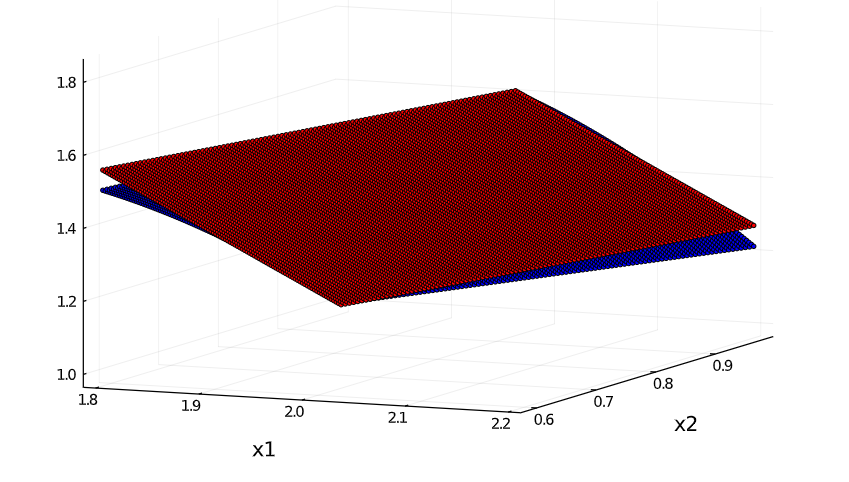
\includegraphics[width=0.48\columnwidth]{Chap11NonlinearEquations/VectorLinearApprox.png}
    }
      %\vspace{.2cm}
\subfloat[]{%
	\centering
  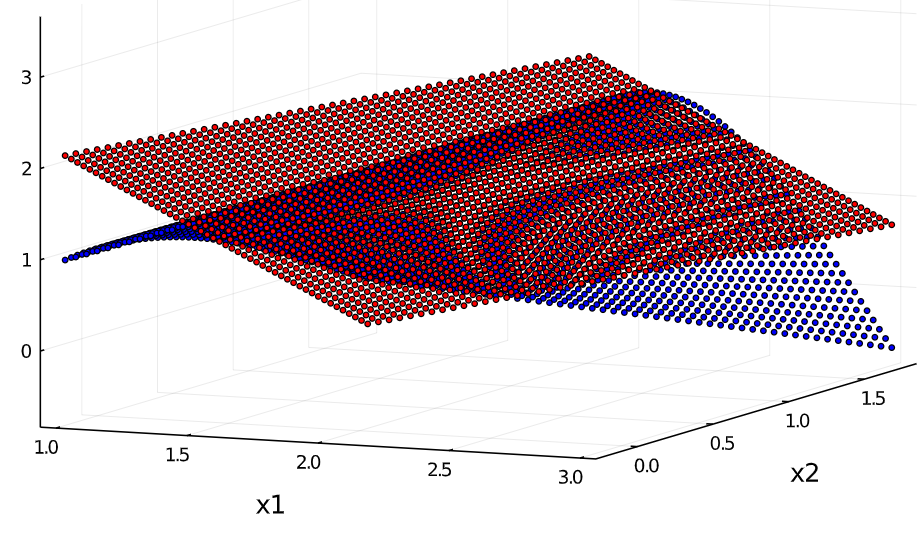
\includegraphics[width=0.48\columnwidth]{Chap11NonlinearEquations/LinearApproximationMoreCurvature.png}
  }
    \caption[]{(a) Close up view. (b) A more global view. The function $f(x_1, x_2) = x_1 \cos(x_2)$ is plotted in blue, while in red is shown its linear approximation about the point $x_0=[2~~\pi/4]^\top$, that is,  $f_{\rm lin}(x) :=f(x_0) + \nabla f(x_0) (x-x_0)$. This approximation can be done for any point $x_0$ at which the partial derivatives exists. In Calculus, the red plane is also called the \textbf{tangent plane at} $\mathbf{x_0}$. These linear approximations accurately represent the nonlinear function in a small enough region about a given point, allowing us to use our Linear Algebra skills. 
    }
    \label{fig:optional:VectorLinearApprox}
    \end{figure}

\vspace*{.2cm}

\begin{example} 
\label{ex:optional:Gradient} 
Compute a linear approximation of $f(x_1, x_2) = x_1 \cos(x_2)$ at the point $x_0=[2~~\pi/4]^\top$.
\end{example}

\textbf{Solution:} From Example~\ref{ex:optional:PartialDerivative}, we know both of the partial derivatives of $f$ at the point $x_0=[2~~\pi/4]^\top$. Hence, we have
\begin{equation}
    \label{eq:optional:gradientExample}
    \begin{aligned}
  f(x) &\approx f(x_0) + \nabla f(x_0) (x-x_0)\\
    &= f(x_0)  + \left[\begin{array}{cc}
        \frac{\partial f(x_0)}{\partial x_1} &  \frac{\partial f(x_0)}{\partial x_2}
    \end{array} \right]  \left[\begin{array}{c}
        x_1-x_{01} \\
        x_2-x_{02} \\
           \end{array} \right]\\
    &= 2 \cos(\pi/4) + \left[
    \begin{array}{cc}
        \frac{\sqrt{2}}{2} & -\sqrt{2}\end{array} \right] \left[\begin{array}{c}
        x_1-2 \\
        x_2-\pi/4 \\
           \end{array} \right]
    \end{aligned}
\end{equation}

Figure~\ref{fig:optional:VectorLinearApprox} compares the linear approximation to the nonlinear function in a region about $x_0$. 
\Qed

\subsection{Expanding on Vector Notation}
\label{sec:optional:optional:optional:CompactDerivativeNotation}

We have carefully defined derivatives and partial derivatives of functions at given points. We used the notation $x_0$ for the given point to make it seem like some concrete value, a fixed scalar in $\real$ of vector in $\real^m$. However, in practice, such as in Newton's Algorithm, we keep updating the point $x_0$ at which we are computing derivatives and linear approximations of functions. Hence, because the point is not really fixed, we can just call it $x$. Then, for $f:\real \to \real$, we have 
\begin{equation}
    \label{eq:optional:betterDerivativeNotation01}
    \frac{df(x)}{dx}\approx \frac{f(x+h) - f(x-h)}{2h},
\end{equation}
and for $f:\real^m \to \real$, where $x=(x_1, x_2, \ldots, x_m)$, we have
\begin{equation}
    \label{eq:optional:betterDerivativeNotation02}
    \frac{\partial f(x)}{\partial x_i}\approx \frac{f(x_1, \ldots, x_i+h, \ldots, x_m) - f(x_1, \ldots, x_i-h, \ldots, x_m)}{2h}.
\end{equation}

With this notation in mind, we now define \textbf{derivatives and partial derivatives for vector valued functions}. When $f:\real \to \real^n$, we have that $x$ is a scalar and $f(x)$ is a vector with $n$ components, as in 
\begin{equation}
    \label{eq:optional:VectorFunctions01}
    f(x) = \left[\begin{array}{c}
       f_1(x) \\
       f_2(x) \\
       \vdots\\
       f_n(x) 
    \end{array} \right].
\end{equation}
We define its derivative with respect to the scalar variable $x$ as
\begin{equation}
    \label{eq:optional:VectorFunctions02}
    \frac{df(x)}{dx} := \left[\begin{array}{c}
      \frac{df_1(x)}{dx} \medskip \\
       \frac{df_2(x)}{dx} \\
       \vdots\\
      \frac{df_n(x)}{dx}
    \end{array} \right],
\end{equation}
by differentiating each of the components of $f(x)$. It's the obvious thing to do. The key is that you must keep track that when $f(x)$ is vector valued, so is its derivative, $ \frac{df(x)}{dx}$. \\

In terms of our symmetric difference approximation to the derivative, the formula,
\begin{equation}
\label{eq:optional:symmetricDifferenceVectorValued}
   \frac{df(x)}{dx}\approx \frac{f(x + h)- f(x-  h)}{2 h},
\end{equation}
is still valid and is even written in Julia the same way! Yes, you could re-write the above as
\begin{equation}
\label{eq:optional:symmetricDifferenceVectorValued02}
   \frac{df(x)}{dx}\approx \left[\begin{array}{c}
     \frac{f_1(x + h)- f_1(x-  h)}{2 h} \medskip \\
      \frac{f_2(x + h)- f_2(x-  h)}{2 h} \\
       \vdots\\
      \frac{f_n(x + h)- f_n(x-  h)}{2 h}
    \end{array} \right],
\end{equation}
 but that's a lot of extra programming. The expression \eqref{eq:optional:symmetricDifferenceVectorValued} is much more compact and convenient. This is the power of good notation.\\

Similarly, when $f:\real^m \to \real^n$, we know that $x$ is a vector with $m$ components and $f(x)$ is a vector with $n$ components, as in 
\begin{equation}
    \label{eq:optional:VectorFunctionsA}
    f(x) = \left[\begin{array}{c}
       f_1(x_1, \ldots, x_m) \\
       f_2(x_1, \ldots, x_m) \\
       \vdots\\
       f_n(x_1, \ldots, x_m) 
    \end{array} \right].
\end{equation}
We define its partial derivative with respect to component $x_i$ as
\begin{equation}
    \label{eq:optional:VectorFunctionsB}
    \frac{\partial f(x)}{\partial x_i} := \left[\begin{array}{c}
      \frac{\partial f_1(x)}{\partial x_i} \medskip \\
       \frac{\partial f_2(x)}{\partial x_i} \\
       \vdots\\
      \frac{\partial f_n(x)}{\partial x_i}
    \end{array} \right],
\end{equation}
by doing the partial differentiation of each of the components of $f(x)$. It's the obvious thing to do. \\

In terms of our symmetric difference approximation to the derivative, the formula,
\begin{equation}
\label{eq:optional:symmetricDifferenceVectorValuedA}
     \frac{\partial f(x)}{\partial x_i}\approx \frac{f(x_1, \ldots, x_i+h, \ldots, x_m) - f(x_1, \ldots, x_i-h, \ldots, x_m)}{2h},
\end{equation}
is still valid and is even written in Julia the same way! Once again, you could re-write the above as
\begin{equation}
\label{eq:optional:symmetricDifferenceVectorValuedB}
  \frac{\partial f(x)}{\partial x_i}\approx \left[\begin{array}{c}
     \frac{f_1(x_1, \ldots, x_i+h, \ldots, x_m) - f_1(x_1, \ldots, x_i-h, \ldots, x_m)}{2h} \medskip \\
      \frac{f_2(x_1, \ldots, x_i+h, \ldots, x_m) - f_2(x_1, \ldots, x_i-h, \ldots, x_m)}{2h}\\
       \vdots\\
      \frac{f_n(x_1, \ldots, x_i+h, \ldots, x_m) - f_n(x_1, \ldots, x_i-h, \ldots, x_m)}{2h}
    \end{array} \right],
\end{equation}
 but that's a lot of extra programming. The expression \eqref{eq:optional:symmetricDifferenceVectorValuedA} is much more compact and convenient. \textbf{This is again the power of good notation. But to use the notation effectively, we have to do the bookkeeping and remember that the innocent expression 
 $$\mathbf{ \frac{\partial f(x)}{\partial x_i} }$$
 is really a vector with $n$ components.} 



\subsection{The Jacobian}

We now turn to functions $f:\real^m \to \real^n$. Based on the compact notation covered in Chapter~\ref{sec:optional:CompactDerivativeNotation}, we can define the \textbf{Jacobian of a function} as
\begin{equation}
    \label{eq:optional:DefJacobian}
    \frac{\partial f(x)}{\partial x}:=  \left[\begin{array}{cccc}
      \frac{\partial f(x)}{\partial x_1} & \frac{\partial f(x)}{\partial x_2} & \cdots & \frac{\partial f(x)}{\partial x_m}
    \end{array} \right].
\end{equation}
Comparing the above to \eqref{eq:optional:GradientDef}, we see that the \textbf{Jacobian} of a function $f:\real^m \to \real$ is the \textbf{gradient} of the function. \textbf{This is the same as saying an $n \times m$ matrix reduces to a row vector when $n=1$. } \\

We need to keep in mind that, for each value of $x\in \real^m$, the compact and innocent looking object
$$ \frac{\partial f(x)}{\partial x} $$
is really an $n \times m$ matrix. When computing it numerically, we typically build it up one column at a time as in the following Julia code.
    
\begin{lstlisting}[language=Julia,style=mystyle]
F(x1,x2,x3)=[x1.*x2.*x3; log.(2+cos.(x1)) .+ x2.^x1; x1.*x3/(1 .+ x2.^2)]
h=0.01
x0=[pi;1.0;2.0]
dfdx1 =(F(x0[1]+h,x0[2],x0[3])-F(x0[1]-h,x0[2],x0[3]))/(2*h)
dfdx2 =(F(x0[1],x0[2]+h,x0[3])-F(x0[1],x0[2]-h,x0[3]))/(2*h)
dfdx3 =(F(x0[1],x0[2],x0[3]+h)-F(x0[1],x0[2],x0[3]-h))/(2*h)
dfdx=[dfdx1 dfdx2 dfdx3]

3x3 Array{Float64,2}:
 2.0   6.28319  3.14159
 0.0   3.14172  0.0
 1.0  -3.14159  1.5708
 \end{lstlisting}
 
 \vspace*{.2cm}

Just for the record, we will write out $\frac{\partial f(x)}{\partial x}$ as an $n \times m$ matrix. In case you are wondering, your instructors never do this when doing real robotics! We use the ``vector version'' of the Jacobian where we compute each column of the matrix. 
For $f:\real^m \to \real^m$, 
\begin{equation}
    \label{eq:optional:VectorFunctions03}
    \frac{\partial f(x)}{\partial x} = \left[\begin{array}{cccc}
      \frac{\partial f_1(x)}{\partial x_1} & \frac{\partial f_1(x)}{\partial x_2} & \cdots & \frac{\partial f_1(x)}{\partial x_m} \medskip \\
      \frac{\partial f_2(x)}{\partial x_1} & \frac{\partial f_2(x)}{\partial x_2} & \cdots & \frac{\partial f_2(x)}{\partial x_m} \medskip \\
      \vdots & \vdots & \ddots & \vdots \medskip \\
      \frac{\partial f_n(x)}{\partial x_1} & \frac{\partial f_n(x)}{\partial x_2} & \cdots & \frac{\partial f_n(x)}{\partial x_m} 
    \end{array} \right].
\end{equation}
Hence, the $ij$ component of $\frac{\partial f(x)}{\partial x}$ is
$\frac{\partial f_i(x)}{\partial x_j}. $
If one wishes, the Jacobian can be computed one element at time via
\begin{equation}
    \label{eq:optional:VectorFunctions03B}
    \frac{\partial f_i(x)}{\partial x_j} \approx \frac{f_i(x_1, \ldots, x_j+h, \ldots, x_m) - f_i(x_1, \ldots, x_j-h, \ldots, x_m)}{2h}. 
    \end{equation}

\begin{tcolorbox}[sharp corners, colback=green!30, colframe=green!80!blue,title={\textbf{From slopes of lines}$\to$\textbf{slopes of functions at points}~$\mathbf{\to \frac{df(x_0)}{dx} \to \nabla f(x_0) \to \frac{\partial f(x_0)}{\partial x}}$}]
Derivatives, gradients, and Jacobians are all generalizations of the notion of the slope  of a line being its ``rise over run''. The derivative of a function $f:\real \to \real$ at a point $x_0$ is the ``local'' slope of the function at that point. We compute it by ``rise over run'', where, for example
\begin{equation}
    \label{eq:optional:SummaryDerivative}
 \text{\rm slope} = \frac{f(x_0+h)-f(x_0)}{h} \xrightarrow[h>0~\text{small}]{} \frac{df(x_0)}{dx},
\end{equation}
and to make it local, we take $h>0$ small. The gradient recognizes that a function $f:\real^m \to \real$ has a local slope in the $x_1$-direction, the $x_2$-direction, all the way up to the $x_m$-direction. If we let $\{e_1, e_2, \ldots, e_m \}$ be the natural basis vectors for $\real^m$, then we compute each component of the gradient by 
\begin{equation}
    \label{eq:optional:SummaryGradient01}
    \text{\rm slope}_j = \frac{f(x_0+h e_j)-f(x_0)}{h}  \xrightarrow[h>0~\text{small}]{} \frac{\partial f(x_0)}{\partial x_j}, 
    \end{equation}
and we assemble the gradient by 
\begin{equation}
    \label{eq:optional:SummaryGradient02}
\nabla f(x_0):= \left[\begin{array}{cccc} \frac{\partial f(x_0)}{\partial x_1} & \frac{\partial f(x_0)}{\partial x_2} & \cdots & \frac{\partial f(x_0)}{\partial x_m}
\end{array} \right]. 
\end{equation}
Finally, for $f:\real^m \to \real^n$, each of the $n$ components of $f(x)$ has a local slope with respect to each component of $x$. The bookkeeping is easiest if we leave $f(x)$ as a vector and write the Jacobian so that it \textbf{looks just like} the gradient,  
\begin{equation}
    \label{eq:optional:SummaryJacobian01}
    \frac{ \partial f(x_0) }{\partial x}:= \left[\begin{array}{cccc} \frac{\partial f(x_0)}{\partial x_1} & \frac{\partial f(x_0)}{\partial x_2} & \cdots & \frac{\partial f(x_0)}{\partial x_m}
\end{array} \right],  
\end{equation}
but now, because $f(x)$ is an $n$-vector, we have 
\begin{equation}
    \label{eq:optional:SummaryJacobian02}
    \left[\begin{array}{c}  \text{\rm slope}_{1j}\\ \vdots \\ \text{\rm slope}_{ij} \\ \vdots \\ \text{\rm slope}_{nj} \end{array}  \right] = \frac{f(x_0+h e_j)-f(x_0)}{h}  \xrightarrow[h>0~\text{small}]{} \frac{\partial f(x_0)}{\partial x_j}. 
\end{equation}
\end{tcolorbox}

\begin{tcolorbox}[title=\textbf{Compact Way to Numerically Approximate the Jacobian}]
If we let $\{e_1, e_2, \ldots, e_m \}$ be the natural basis vectors for $\real^m$, then a more compact notation allows us to compute each column of the Jacobian by 
\begin{equation}
    \label{eq:optional:SummaryGradient01A}
    \frac{\partial f(x_0)}{\partial x_j} = \frac{f(x_0+h e_j)-f(x_0)}{h}.
    \end{equation}
    Typically, this is easier to program up than \eqref{eq:optional:VectorFunctions03B}. But of course, your experience may vary! For a symmetric difference, we'd use
    \begin{equation}
    \label{eq:optional:SummaryGradient01B}
    \frac{\partial f(x_0)}{\partial x_j} = \frac{f(x_0+h e_j)-f(x_0- h e_j)}{2h}.
    \end{equation}
\end{tcolorbox}

\subsection{Linear Approximation of Vector Valued Functions}

 Our goal remains to build linear approximations of the form $f(x) \approx f(x_0) + A ( x - x_0)$. Just as with our previous investigations, the matrix $A$ is associated with derivatives of the function. In fact, we have 
 \begin{equation}
     \label{eq:optional:VectorJacobianBasedLinearApprox}
     f(x) \approx f(x_0) + \underbrace{\frac{\partial f(x_0)}{\partial x}}_{A}  ( x - x_0),
 \end{equation}
 in other words, $A:=\left. \frac{\partial f(x)}{\partial x}\right|_{x=x_0}$.\\
 
 \begin{example}
 \label{ex:optional:JacobianBasedApproximation}
 For the function 
 \begin{equation}
 f(x_1,x_2,x_3):= 
 \left[
\begin{array}{c}
x_1 x_2 x_3  \\
\log(2+\cos(x_1)) + x_2^{x_1} \\
 \frac{x_1 x_3}{1+ x_2^2} \\
\end{array}
\right],
 \end{equation}
 compute its Jacobian at the point 
 $$x_0 = \left[
\begin{array}{c}
\pi \\
1.0 \\
2.0 \\
\end{array}
\right]$$
and evaluate the ``accuracy'' of its linear approximation.
  \end{example}
 
 \textbf{Solution}
 Using Symmetric Differences, the Jacobian at $x_0$ is 
 \begin{equation}
 A=\frac{\partial f(x_0)}{\partial x}\approx
\left[
\begin{array}{rrr}
2.00 & 6.28 & 3.14 \\
0.00 & 3.14 & 0.00 \\
1.00 & -3.14 & 1.57 \\
\end{array}
\right]
\end{equation}
 
 Figure~\ref{fig:optional:VectorLinearApprox} is the limit of what we can show in plots. Another way to think about the question of assessing the quality of the linear approximation is to measure the error defined as
 $$e(x):= ||f(x)-f_{\rm lin}(x) ||,$$
 where $f_{\rm lin}(x):=f(x_0) + \frac{\partial f(x_0)}{\partial x} (x - x_0)$. We will seek to estimate the maximum value of $e(x)$ over a region containing the point $x_0$.
 Define 
 $$S(x_0):= \{x  \in \real^3 ~|~~~ |x_i-x_{0i} | \le d, i=1,2,3 \} $$
 and 
\begin{equation}
    \label{eq:optional:MaxErrorLinApprox}
    {\rm Max~~ Error} := \max_{x\in S(x_0)} e(x) = \max_{x\in S(x_0)} ||f(x)-f_{\rm lin}(x) ||.
\end{equation}
The for $d=0.25$, we used a ``random search'' routine and estimate that
$$ {\rm Max~~ Error}=0.12.$$
To put this into context, 
$$  \max_{x\in S(x_0)} ||f(x)|| = 8.47,$$
and thus the relative error is about $1.5\%.$
\Qed

If you made it to here, you should loop back to Chap.~\ref{sec:Newtonraphson}. 

\section{Looking Ahead}

We've seen that an interesting idea from Calculus, called the derivative, allows nonlinear functions to be approximated by linear functions. The matrices resulting from a derivative, gradient, or Jacobian were instrumental in building algorithms to find roots of nonlinear equations.\\

In this next Chapter, we'll use the derivative and the gradient to understand algorithms for finding a minimum or a maximum of a function. We'll be able to greatly extend the ideas we developed in Chapters~\ref{sec:LeastSqauresGeneral} for least squared error solutions to $Ax=b$ when it had no solutions, Chapter~\ref{sec:LinearRegression} for regression of functions to data, and Chapter~\ref{sec:MinNormSolution2LinearEquations}, where we were able to identify a unique solution of minimum norm when $Ax=b$ had an infinite number of solutions.